\RequirePackage{fix-cm}

\documentclass[smallextended,natbib]{svjour3}

\smartqed

\usepackage{graphicx}

%\usepackage[left=2.5cm,top=3.5cm,right=2.5cm,bottom=2cm,nohead]{geometry}

\usepackage[english]{babel}
\usepackage[utf8]{inputenc}
%\usepackage{cite}
%\usepackage{natbib}
\usepackage[T1]{fontenc}  
\usepackage{hyperref}  
\usepackage{algpseudocode}
\usepackage{algorithm}
\usepackage{textcomp}
\floatstyle{plain}
\newfloat{myalgo}{tbhp}{mya}
\usepackage{bm}
\usepackage{pdflscape}
\usepackage{rotating}
\usepackage{enumerate}
\usepackage{subfigure}
\usepackage{setspace}
%\usepackage{float}
%\usepackage[usenames, dvipsnames]{color, colortbl}
\usepackage{pbox}
\usepackage{color}
\usepackage[table]{xcolor}  
\usepackage{tabu}
\usepackage{verbatim}
\usepackage{amsmath}
\usepackage{amssymb}
\usepackage{latexsym}
\usepackage{multirow}
\usepackage{array}
\usepackage{makecell}
%\setcellgapes{1.25pt}

%\usepackage{dsfont}

\usepackage{caption}

\definecolor{darkblue}{rgb}{0.0, 0.0, 0.55}

%\captionsetup[lstlisting]{font={footnotesize, bfseries}}

%\usepackage[margin=1.0in]{geometry}% http://ctan.org/pkg/margin
\usepackage{booktabs}% http://ctan.org/pkg/booktabs
\usepackage{array}% http://ctan.org/pkg/array

\usepackage{colortbl}
\newcolumntype{C}{r<{\kern\tabcolsep{\hspace{10pt}}}}

\usepackage{listings}
\usepackage{fancy-listings}

\definecolor{bostonuniversityred}{rgb}{0.8, 0.0, 0.0}
\definecolor{blue(pigment)}{rgb}{0.2, 0.2, 0.6}
\definecolor{verdeescuro}{rgb}{0.0, 0.44, 0.0}

\lstset{
language=Java,
numbers=left,
frame=shadowbox,
basicstyle=\ttfamily\footnotesize,
captionpos=b,
boxpos=c,
lineskip={-1.5pt},
moredelim=**[is][\color{bostonuniversityred}]{@}{@},
moredelim=**[is][\color{blue(pigment)}]{|}{|},
moredelim=**[is][\color{verdeescuro}]{&}{&},
%xleftmargin=0.3cm,
%xrightmargin=0.3cm,
}

\renewcommand\lstlistingname{Code}
\renewcommand\lstlistlistingname{Codes}

%\usepackage{amsmath}

\newenvironment{Algorithm}[2][tbh]%
{\begin{myalgo}[#1]
\centering
\begin{minipage}{#2}
\begin{algorithm}[H]}%
{\end{algorithm}
\end{minipage}
\end{myalgo}}

\newcommand{\bigO}{\ensuremath{\mathcal{O}}}
\newcommand{\subscript}[1]{\ensuremath{_{\textrm{#1}}}}
\newcommand{\aspas}[1]{{``#1''}}

\newcommand{\tab}{\text{}\text{}\text{}}

\newcommand{\classeremovida}{%
\pbox{0.8cm}{\setstretch{0.7}\centering\textcolor{Gray}{\tiny classe removida}}%
}

\newcommand{\novaclasse}{%
\pbox{0.9cm}{\centering\textcolor{Gray}{\tiny nova classe}}%
}

\newcommand{\aspassimples}[1]{{`#1'}}

\newcommand{\scode}[1]{{$\scriptstyle{#1}$}}
\newcommand{\code}[1]{{$\texttt{#1}$}}
\newcommand{\mcode}[1]{{$\mathtt{#1}$}}

\newcolumntype{P}[1]{>{\centering\arraybackslash}p{#1}}

\definecolor{darkgreen}{rgb}{0.0, 0.2, 0.13}
\definecolor{darkolivegreen}{rgb}{0.33, 0.42, 0.18}
\definecolor{olivine}{rgb}{0.6, 0.73, 0.45}
\definecolor{mycolor}{rgb}{0.64, 0.76, 0.68}
\definecolor{cambridgeblue}{rgb}{0.64, 0.76, 0.68}
\sloppy
\begin{document}

\title{Better Similarity Coefficients to Identify Refactoring Opportunities}

\author{Arthur F. Pinto \and
	Ricardo Terra
}

\institute{Arthur F. Pinto \at
Computer Science Department, Universidade Federal de Lavras (UFLA), Brasil\\
\email{fparthur@posgrad.ufla.br} 
\and
Ricardo Terra \at
Computer Science Department, Universidade Federal de Lavras (UFLA), Brasil\\
\email{terra@dcc.ufla.br}
}

\date{Received: date / Accepted: date}

\maketitle

\begin{abstract}
Similarity coefficients are used by several techniques to identify refactoring opportunities. As an example, it is expected that a method is located in a class that is structurally similar to it. However, the existing coefficients in Literature have not been designed for the structural analysis of software systems, which may not guarantee satisfactory accuracy. This article, therefore, proposes new coefficients---based on genetic algorithms over a training set of 10 systems---to improve the accuracy of the identification of Move Class, Move Method, and Extract Method refactoring opportunities. We conducted an empirical study comparing these proposed coefficients with other 18 coefficients in other 101 systems. The results indicate, in relation to the best analyzed coefficient, a statistical improvement \textcolor{black}{from 5.23\% to 6.81\% for the identification of Move Method refactoring opportunities, 12.33\% to 14.79\% for Move Class, and 0.25\% to 0.40\% for Extract Method}. Moreover, we implemented a tool that relies on the proposed coefficients to recommend refactoring opportunities.
\keywords{Software Architecture \and Structural Similarity \and Code Refactoring \and Move Class \and Move Method \and Extract Method}
\end{abstract}

\section{Introduction}
\label{sec:intro}

During software development, the software architecture is subjected to several problems. Code Smells (also called Bad Smells) are defined as any symptoms in the code that might indicate one of these problems~\citep{fowler1999refactoring}. Frequently, such Code Smells imply in the establishment of unnecessary dependencies. However, considering that ensuring architectural design is extremely important for maintainability, reusability, scalability, and portability of software systems~\citep{leoterr}, it is expected that the code elements of a software project be located in structurally similar entities.

%It should be noted that this article takes into consideration structural dependencies among the code elements of a system for similarity calculation among packages, classes, methods and blocks. Structural dependencies occur when a compilation unit depends on another in relation to compile time or link time~\citep{fow03}. Among the several types of dependency that exist in an object-oriented programming, it can be mentioned as more relevant: method and attribute access (\textit{access}), variable declaration (\textit{declare}), object creation (\textit{create}), class extension (\textit{extend}), interface implementation (\textit{implement}), exception activation (\textit{throw}) and use of annotations (\textit{useannotation}).

%A code structure with good similarity indexes directly influences software quality, since it evidences the high cohesion degree and low coupling, positively affecting the software architecture and maintenance characteristics.

In order to ensure the structural similarity among code entities and to avoid the occurrence of Code Smells, it must be verified the similarity of dependencies among its elements (whether in the level of package, class, method or block), besides performing refactorings when necessary. This implies moving methods and classes, and in the extraction of a code block from a method (generating a new method), through refactorings like \textit{Move Class}, \textit{Move Method} and \textit{Extract Method}~\citep{fowler1999refactoring}.

%Para maior compreensão, a
Figure~\ref{fig:intro} shows an example of a system that follows the MVC architecture, consisting of three layers: $Model$, $View$ and $Controller$. It is possible to note that $C_2$ is badly located in the $Controller$ layer since it depends on graphical elements while other classes of the layer have dependencies to manipulation elements of request and answers (e.g., \mcode{HttpRequest} e \mcode{HttpResponse}). Therefore, it is possible to suggest moving such class (\textit{Move Class}) to a structurally similar layer that, in this scenario, would be the $View$ layer. Such structural similarity occurs because $C_2$ and classes from the $View$ layer ($V_1, \dots, V_n$) have dependencies on common graphical elements (e.g., \mcode{JPanel} and \mcode{JLabel}). Thus, refactoring would not only guarantee an architecture with properly located entities, but would also respect the MVC architecture.

\begin{figure}[ht]
\centering
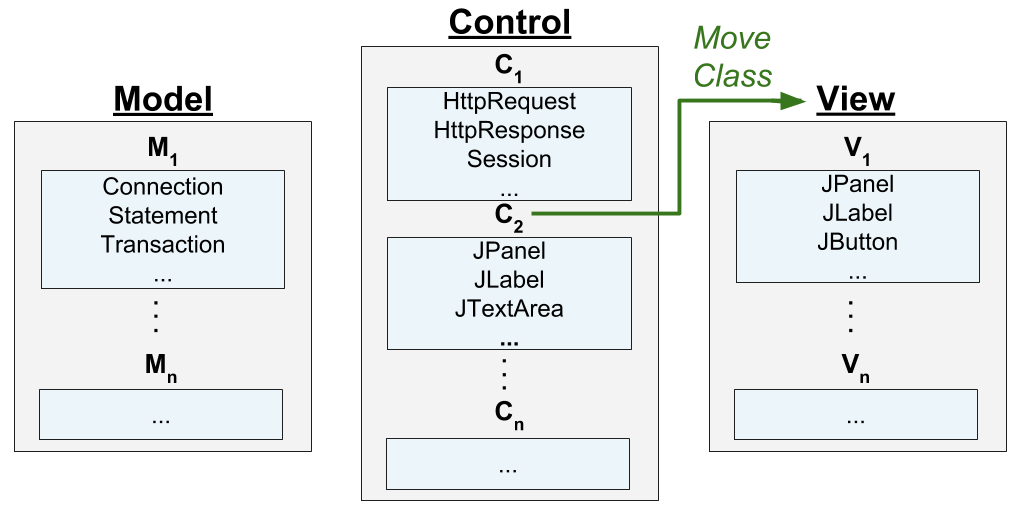
\includegraphics[scale=0.26]{exemintro.png}
\caption{Move Class Refactoring Example}
\label{fig:intro}
\vspace{-0.5cm}
\end{figure}

Several coefficients were proposed for the calculation of similarity among code entities. However, the use of such coefficients may not guarantee satisfactory accuracy. Moreover, the main current coefficients in the literature were not designed for the structural analysis of a software system. For instance, the \textit{Jaccard} coefficient, one of the most used in Software Engineering, was initially designed to compare the similarity among flower species in different districts~\citep{jaccard1912}.

%\textcolor{red}{***MELHORAR AS EXISTENTES***}
Therefore, this article aims primarily to propose new similarity coefficients for a more precise identification of {\textit{Move Class}, \textit{Move Method} and, \textit{Extract Method} refactoring opportunities .
%Além disso, é importante ressaltar que a abordagem utilizada neste artigo é exclusiva para esses tipos de refatoração.}
This makes it possible to (i)~locate more accurately entities improperly positioned on a system architecture and (ii)~leverage the accuracy of tools for identification of refactoring opportunities based on structural similarity. It is important to emphasize, however, that the new coefficients are specific to these three refactorings, since they are the most widely used by developers~\citep{silva2016we}.

Firstly,we investigated the accuracy of 18 similarity coefficients in 10 systems (training set) of \textit{Qualitas.class Corpus}~\citep{qc}.
%
Secondly, we adapted the \textit{Simple Matching} coefficient through genetic algorithms in order to generate three new coefficients ($PTMC$, $PTMM$ e $PTEM$) with greater precision in the identification of \textit{Move Class}, \textit{Move Method}, and \textit{Extract Method} refactoring opportunities, respectively. 
%
Thirdly, we compared the proposed coefficients with those existent in other 101 systems. The results indicate, in relation to the best analyzed coefficient, \textcolor{black}{a statistically significant improvement from 5.23\% to 6.81\% for identification of \textit{Move Method} opportunities, 12.33\% to 14.79\% for \textit{Move Class}, and 0.25\% to 0.40\% for \textit{Extract Method}}. 
Finally, we implemented a tool that identifies refactoring opportunities based on the proposed coefficients.

\textcolor{black}{This article is an extended version of our first work on our first work on proposing such coefficients~\citep{2017_sbcars} where we highlight the following improvements: (i)~an adaptation in the proposal of the coefficients, where exponents weights and more concise numbers are applied in their formulas; (ii)~the introduction of a new experiment in the methodology to ensure better results of the adapted coefficients; (iii)~an improved analysis of the results, addressing the problem that some data do not follow a normal distribution; (iv)~new results, with higher precision of the proposed coefficients, thus more efficient; and (v)~a more complete and detailed tool section.}

The remainder of this article is organized as described below. Section~\ref{sec:background} introduces fundamental concepts to the study. Section~\ref{sec:metodologia} describes the used methodology. Section~\ref{sec:analise} presents an analysis of existing coefficients, with the objective of selecting the coefficient to be adapted. Section~\ref{sec:proposta} proposes three new coefficients for identifying refactoring opportunities. Section~\ref{sec:avaliacao} shows an evaluation of the proposed coefficients in 101 systems. Section~\ref{sec:sistema} describes the implementation of a tool to identify refactoring opportunities based on the proposed coefficients. Section~\ref{sec:trabrela} discusses related studies. Finally, Section~\ref{sec:conclusao} presents the final considerations and future research.

\section{Background}
\label{sec:background}
In order to provide the necessary knowledge for the conception and understanding of this article, we introduce the fundamental concepts. Section~\ref{sec:refatoracao} deals with the refactoring process, which involves methods for source code restructuring. Section~\ref{sec:similaridade} deals with structural similarity, as also presents the current main coefficients in the literature. Section~\ref{sec:algooti} introduces optimization algorithms, focusing on genetic algorithms, besides presenting an illustrative example of optimization. %\textcolor{black}{Finally, Section~\ref{sec:reftuk} describes an adaptation of \textit{Tukey's Test} used as an approach in this article.}

\subsection{Refactoring}
\label{sec:refatoracao}

Code refactoring is the process of moving a software system in a way that preserves the external code behavior while improves its internal structure~\citep{fowler1999refactoring}. Through the refactoring, it becomes possible to treat the occurrence of different Code Smells.
%
Although some refactoring processes consider other aspects (e.g., semantics), the present study focuses exclusively on Code Smells structurally manifested in the source code.

Several techniques can be used for code refactoring. Considering that this article focuses its analysis exclusively on classes, methods, and blocks of a system, the \textit{Move Class}, \textit{Move Method}, and \textit{Extract Method} refactorings will be used in order to address the occurrence of Code Smells. Whereas the application of  \textit{Move Class} and \textit{Move Method} consists, respectively, in the simple movement from a class to another package and in the movement from a method to another class,  \textit{Extract Method} is accomplished through the extraction from a code block to a new method that will be generated by replacing the extracted fragment with a call to the new referred method.

Although the application of \textit{Move Class} for repositioning a class in its due package does not address any specific Code Smell, it is fundamental to avoid the occurrence of any Code Smell since the undue location of a class will contribute to its inadequate internal structure, i.e., it will result in inappropriately positioned methods and blocks.

However, the \textit{Move Method} makes possible treating the following Code Smells: \textit{Large Class}, in which the repositioning of undue methods will reduce the size of the referred class; \textit{Divergent Change} and \textit{Shotgun Surgery}, in which it will be possible to position methods that need changes in a specific class that does not cause the need for changes; \textit{Feature Envy}, in which methods that overuse internal properties from another class can be moved to the other referred class; and \textit{Refused Bequest}, where superclass methods, which do not have properties in common with all subclasses, can be moved to the subclasses that use them.

The \textit{Extract Method} refactoring, in turn, provides means of dealing with \textit{Long Method}, in which extracting code blocks into new methods will reduce the size of the referred method. Furthermore, although \textit{Extract Method} deals only directly with \textit{Long Method}, it can indirectly be used to treat other Code Smells (e.g., \textit{Large Class}, \textit{Divergent Change}, \textit{Shotgun Surgery}, \textit{Feature Envy}, and \textit{Refused Bequest}) since after extracting the code block in a new method, this one can be moved to another class through \textit{Move Method}. In this way, the referred Code Smells can be handled in situations where they occur in only certain code blocks.

\subsection{Structural Similarity}
\label{sec:similaridade}
In order to identify the occurrence of Code Smells and hence code refactoring opportunities, it is primordial to analyze the structural similarity of the code entities present in a software design. Similarity, in the context of software architecture, deals with the relationship between shared properties between two or more entities present in the code structure.

For the calculation of similarity indices, %several coefficients were proposed.
Table~\ref{tab:table1} reports the main similarity coefficients proposed in the literature~\citep{2013_seke}.\\[-0.7cm]

\begin{table}[ht]
\caption{Similarity Coefficients}
\vspace{-8pt}
\centering
%\scriptsize
\footnotesize
\label{tab:table1}
%\resizebox*{\linewidth}{0.24\textheight}{%
\begin{tabular}{p{3.6cm}p{5.5cm}p{0.9cm}}
\hline %\hline %\hline\noalign{\smallskip}
\rowcolor{gray!25} {\bf Coefficient} & {\bf Definition} & {\bf Range}\\
\hline %\hline %\noalign{\smallskip}\hline %\hline\noalign{\smallskip}
\rowcolor{white} \mbox{Baroni-Urbani and Buser} & \mcode{[a + (ad)^{\frac{1}{2}}]/[a + b + c + (ad)^{\frac{1}{2}}]} & [0-1*]  \\
\rowcolor{gray!15} Dot-product & \mcode{a/(b + c + 2a)} & [0-1*]  \\ 
\rowcolor{white}Hamann & \mcode{[(a + d) - (b + c)]/[(a + d)+(b + c)]} & [-1-1*]  \\
\rowcolor{gray!15}Jaccard & \mcode{a/(a + b + c)} & [0-1*] \\
\rowcolor{white}Kulczynski & \mcode{\frac{1}{2}[a/(a + b) + a/(a + c)]} & [0-1*]  \\ 
\rowcolor{gray!15}Ochiai & \mcode{a/[(a + b)(a + c)]^{\frac{1}{2}}} & [0-1*]  \\ 
\rowcolor{white}Phi & \scriptsize\mcode{(ad - bc)/[(a + b)(a + c)(b + d)(c + d)]^{\frac{1}{2}}} & [-1-1*]  \\ 
\rowcolor{gray!15}PSC & \mcode{a^{2}/[(b + a)(c + a)]} & [0-1*]  \\
\rowcolor{white}Relative Matching & \mcode{[a + (ad)^{\frac{1}{2}}]/[a + b + c + d + (ad)^{\frac{1}{2}}]} & [0-1*]  \\
\rowcolor{gray!15}Rogers and Tanimoto & \mcode{(a + d)/[a + 2(b + c) + d]} & [0-1*]  \\ 
\rowcolor{white}Russell and Rao & \mcode{a/(a + b + c + d)} & [0-1*]  \\ 
\rowcolor{gray!15}Simple Matching & \mcode{(a + d)/(a + b + c + d)} & [0-1*]  \\
\rowcolor{white}Sokal and Sneath & \mcode{2(a + d)/[2(a + d) + b + c]} & [0-1*]  \\ 
\rowcolor{gray!15}Sokal and Sneath 2 & \mcode{a/[a + 2(b + c)]} & [0-1*]  \\ 
\rowcolor{white}Sokal and Sneath 4 & \tiny\mcode{\frac{1}{4}[a/(a + b) + a/(a + c) + d/(b + d) + d/(c + d)]} & [0-1*]  \\
\rowcolor{gray!15}Sokal binary distance & \mcode{[(b + c)/(a + b + c + d)]^{\frac{1}{2}}} & [0*-1]  \\ 
\rowcolor{white}Sorenson & \mcode{2a/(2a + b + c)} & [0-1*]  \\ 
\rowcolor{gray!15}Yule & \mcode{(ad - bc)/(ad + bc)} & [0-1*]  \\ 
\hline %\hline %\noalign{\smallskip}\hline
\\[-0.2cm]
\rowcolor{white} \multicolumn{2}{@{}l}{The * symbol indicates the maximum similarity}
\end{tabular}
%}
\vspace{-0.5cm}
\end{table}

For the understanding of each similarity coefficient, consider two code entities $A$ and $B$. Taking into consideration that this article analyzes structural dependencies among code entities, it has the following variables:\\[-0.2cm]

\tab\textbf{a} = number of dependencies in both entities,\\[-0.4cm]

\tab\textbf{b} = number of exclusive dependencies of entity $A$,\\[-0.4cm]

\tab\textbf{c} = number of exclusive dependencies of entity $B$, and\\[-0.4cm]

\tab\textbf{d} = number of the remainder from the total dependencies considered.\\[-0.2cm]

In order to illustrate the calculation of structural similarity between two code entities, we applied the \textit{Jaccard} and \textit{Simple Matching} coefficients in two methods of the system MyAppointments, a system of control and management of commitments~\citep{leoterr}. In this way, we selected methods \mcode{loadAppointments}, responsible for loading appointments of the system, and \mcode{getAppointmentRowAsDate}, responsible for returning the appointment date of a specific row in the data set. Both methods are present in the same control class. Code~\ref{algo1} shows the implementation of both methods.\\[-0.2cm] % \mcode{loadAppointments} and \mcode{getAppointmentRowAsDate}.\\[-0.2cm]

Based on the analysis of both methods and the structural dependencies present in their structures, it has:

\begin{itemize}
    \item $a = 2$, since both methods access methods from \mcode{AgendaView} and \mcode{DateUtils} (highlighted by red color);\\
    \item $b = 4$, since method \mcode{loadAppointments} has the following exclusive dependencies: the throw of an exception of type \mcode{Exception}, the declaration of \mcode{List} and \mcode{Appointment}, and the access to methods from \mcode{AgendaDAO} (highlighted by blue color);
\end{itemize}
%\begin{center}

\begin{lstlisting} [caption={\mcode{\textbf{AgendaController}} Fragment}, label=algo1,emph={[2]},emphstyle={[2]\bfseries\color{darkblue}}]
public class AgendaController
   ...
   
   public void loadAppointments() throws |Exception| {
      |List|<|Appointment|> apps = |agendaDAO|.getAppointments
         (@DateUtils@.getCurrentDay(), 
      		@DateUtils@.getCurrentMonth(), 
			@DateUtils@.getCurrentYear());
						       
      int i = 0 ;
      for(|Appointment| app : apps) {
         @agendaView@.insertAppointRow
            (i, @DateUtils@.toString(
               app.getDate(), 
               @DateUtils@.HOUR_FMT), 
               app.getTitle());
         i++ ;
      }
   }

   private &Date& getAppointmentRowAsDate(int row) {
      String[] appHour = 
      	@agendaView@.getAppointmentRow(row)[0].split(":");
      return DateUtils.newDate
         (@DateUtils@.getCurrentDay(),
            @DateUtils@.getCurrentMonth(),
            @DateUtils@.getCurrentYear(),
            Integer.parseInt(appHour[0]),
            Integer.parseInt(appHour[1]));        
   }
}
\end{lstlisting}
%\end{center}

\begin{itemize}
    \item $c\hspace{-20pt}=\hspace{-20pt}1$, since the exclusive dependency of the method\hspace{20pt} \mcode{getAppointmentRowAsDate} is the declaration of type \mcode{Date} as return (highlighted by green color);\\
    \item $d = 32$, since when considering the entire system, another 32 types are used by other system entities.
\end{itemize}

It should be noted that dependencies to primitive types (e.g., \mcode{int}, \mcode{char}, \mcode{byte}, etc.), to wrappers classes (e.g., \mcode{Integer}, \mcode{Long}, \mcode{Character}, etc.) and \mcode{String} type are disregarded during the analysis since almost all classes establish dependencies with these types, not contributing to the similarity calculation.

Therefore, when applying, as example, the \textit{Jaccard} and \textit{Simple Matching} coefficient, the following similarity indexes are found:\\
\begin{equation}
\label{eq:simJac}
\footnotesize
\textit{Jaccard} \texttt{ = } \frac{\texttt{$a$}}{\texttt{$a$} \texttt{ + } \texttt{$b$} \texttt{ + } \texttt{$c$}} \texttt{ = } \frac{\texttt{2}}{\texttt{2} \texttt{ + } \texttt{4} \texttt{ + } \texttt{1}} \texttt{ = } \texttt{ 0.28 }
\end{equation}

\begin{equation}
\label{eq:simSM}
\footnotesize
\textit{Simple Matching} \texttt{ = } \frac{\texttt{$a$} \texttt{ + } \texttt{$d$}}{\texttt{$a$} \texttt{ + } \texttt{$b$} \texttt{ + } \texttt{$c$} \texttt{ + } \texttt{$d$}} \texttt{ = } \frac{\texttt{2} \texttt{ + } \texttt{32}}{\texttt{2} \texttt{ + } \texttt{4} \texttt{ + } \texttt{1} \texttt{ + } \texttt{32}} \texttt{ = } \texttt{ 0.87 }
\\[0.15cm]
\end{equation}

Thus, it is important to mention that only the gross value does not indicate the similarity level with accuracy since it is necessary to observe and compare the other similarity values of the system altogether. For instance, 0.28 (\textit{Jaccard}) can be considered a high similarity value if the mean similarity of the system is 0.12. Similarly, 0.87 (\textit{Simple Matching}) can be considered as a low value, depending from the other values.

\subsection{Optimization Algorithms}
\label{sec:algooti}

Optimization refers to the process of finding and comparing solutions to a given problem, maximizing and/or minimizing the values of the variables that compose the objective function until the best possible solution is found~\citep{livrooptimi}. However, in many cases, a problem does not have an optimal solution, which results in the search for solutions that meet the desired objective satisfactorily. This concept, in turn, can be applied to adapt and improve the similarity coefficients discussed in the previous section.

When searching solution of optimization problems, several approaches can be applied, involving different types of algorithms. Among the several approaches, the application of a simple genetic algorithm has shown to be able to find satisfactory solutions effectively. Therefore, it has become the chosen approach for application in this article.

\subsubsection{Genetic Algorithms}
\label{sec:algogen}

A genetic algorithm defines a set of candidates for the proposed solution and, at each iteration (each generation of the genetic algorithm), selects and combines the most suitable candidates, which may undergo slight changes. Thus, at the end of all execution, the solution set will consist of candidates with relative great potential to optimize the objective function~\citep{algogen}. 

Considering the problem of optimizing similarity coefficients, the algorithm defines weights and exponents for each variable of the chosen coefficient formula and each iteration seeks to adapt each weight and exponent in order to optimize the result of the objective function, finally selecting the set of best results. For instance, considering the \textit{Jaccard} coefficient (presented in Table~\ref{tab:table1}), and the weights $P_{a'}$, $P_{a''}$, $P_b$ and $P_c$, \textcolor{black}{as also the exponents $E_{a'}$, $E_{a''}$, $E_b$, and $E_c$,} corresponding, respectively, to variables $a$ of the numerator and $a$, $b$ and $c$ of the denominator. Thus, it has as a result:\\[-0.5cm]

\begin{equation}
\label{eq:coefres}
\footnotesize
\textit{Resulting Coefficient}  \texttt{ = }  \frac{P_{a'} \texttt{ * } \texttt{a'}^{E_{a'}}}{P_{a''} \texttt{ * } \texttt{a''}^{E_{a''}}  \texttt{ + }  P_b \texttt{ * } \texttt{b}^{E_b}  \texttt{ + }  P_c \texttt{ * } \texttt{c}^{E_c}}\\
\\[0.3cm]
\end{equation}

During the execution of a genetic algorithm, the parameters are defined, such as objective function (or fitness function), initial population, number of generations, selection operator, crossover operator, and mutation operator. The objective function represents the data or function to be optimized. The initial population stipulates the initial number of possible candidates for the desired weights \textcolor{black}{and exponents} in order to optimize the objective function. Number of generations refers to the number of times the genetic algorithm will be repeated, i.e., iterate by adapting the desired \textcolor{black}{values}. The selection operator will choose candidates that are more likely to cross-check between them, thus generating one or more candidates who may show more suitability to the solution set. Finally, the generated candidate(s) may undergo a slight mutation, i.e., a slight change in its value, which prevents its stagnation, besides allowing it arriving at any point of the search space.

Among the different operators of selection, crossing and mutation, this article uses, respectively, \textit{Binary Tournament}, \textit{Simulated Binary Crossover}, and \textit{Polynomial Mutation}. %, devido a simplicidade e eficácia dos mesmos.
The \textit{Binary Tournament} method selects, among all the possible generated candidates until then, two individuals that present higher results in relation to the objective function so that they are crossed. The \textit{Simulated Binary Crossover} occurs through the crossing of two individuals, combining their binary representations, in order to generate two new individuals. Such a combination considers a defined probability, analyzing whether each binary index should be combined or not. Finally, the \textit{Polynomial Mutation} also considers a defined probability in order to change one or more binary indexes of the individuals resulting from the crossover. In both crossover and mutation operators, a distribution index must be established in order to evaluate the diversity of the selected solutions in search space, which guarantees the selection of more heterogeneous individuals.

\subsubsection{Illustrative Example}
\label{sec:exemilus}

For a better understanding of the approach of optimization algorithms and concepts of genetic algorithms, this section presents the application of a genetic algorithm to optimize the \textit{Jaccard} similarity coefficient in a little example of \textit{Move Class} refactoring.

For instance, take as assumption a system with two packages $pkg1$ and $pkg2$ with a set of classes and their dependencies, respectively, as $pkg1$~=~\{$A$=\{X,Y,W,Z\}, $B$=\{X,Y,Z,L\}, $C$=\{X,Y,W,K\}\} and $pkg2$~=~\{$D$=\{X,W,R,T\}, $E$=\{R,T,Z\}, $F$=\{X,Z,R,T,M\}\}, according to Figure~\ref{fig:moveeee}.\\[-0.5cm]

\begin{figure}[!ht]
\centering
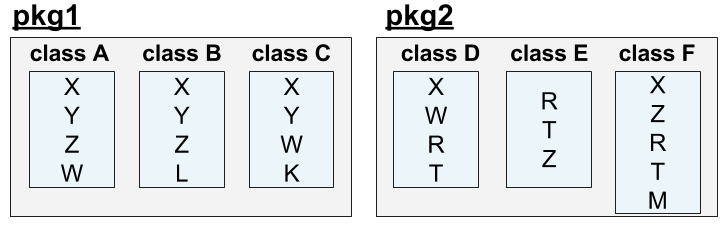
\includegraphics[scale=0.3]{exemilus.png}
\caption{Illustrative Example}
\label{fig:moveeee}
\vspace{-0.5cm}
\end{figure}

Assume it is known that the current system architecture is the ideal one and we intend to use a similarity coefficient in which does not result in suggestions of \textit{Move Class} refactoring, i.e., maintain the current architecture and guarantee good similarity indexes among classes from the same package. To this end, it is intended to adapt a coefficient in order to maximize the similarity of $sim(A,B)$, $sim(A,C)$, $sim(B, C)$, $sim(D,E)$, $sim(D,F)$, and $sim(E,F)$. Simultaneously, it is expected to minimize the similarity $sim(A,D)$, $sim(A,E)$, $sim(A,F)$, $sim(B,D)$, $sim(B,E)$, $sim(B,F)$, $sim(C,D)$, $sim(C,E)$, and $sim(C,F)$. However, only the gross value does not indicate the similarity level with accuracy since it is necessary to observe and compare the other similarity values of the system altogether. In this way, it is intended obtaining the largest possible difference between the arithmetic mean of similarities aimed to maximize and to minimize.

Considering the \textit{Jaccard} coefficient as an example, it is decided to apply the genetic algorithm defining weights \textcolor{black}{and exponents} for each coefficient variable, as previously described in Equation~\ref{eq:coefres}. In this way, we relied on the configurations presented in Table~\ref{tab:conf1}, which was obtained after a series of attempts aimed to improve the coefficients, considering the computational resource disposition and execution time.

\begin{table}[ht]
\centering
\caption{Genetic Algorithms Configuration}
\label{tab:conf1}
\vspace{-8pt}
\scriptsize
%\resizebox{\linewidth}{!}{%
%\begin{tabular}{@{}llll@{}}
%\begin{tabular}{p{50.5pt}lp{50.5pt}@{\hspace{6pt}}lll@{}}
\begin{tabular}{m{95.5pt}>{\centering\arraybackslash}m{80.5pt}m{80.5pt}>{\centering\arraybackslash}m{35.5pt}}
%\tabucline[1.5pt]{-}
\hline %\hline %\noalign{\smallskip}\hline %\hline\noalign{\smallskip}
\rowcolor{gray!15}\textbf{Objective function:} & Number of optimized similarities &
\textbf{Crossover operator:} & Simulated Binary Crossover \\
\rowcolor{white}\textbf{Population size:} & 1200 &
\textbf{Probability of mutation:} & 0.6  \\ %\hline
\rowcolor{gray!15}\textbf{Representation of the population:} & \mbox{$\{x \in \mathbb{R} \mid -2 \leq x \leq 2\}$} 
& 
\textbf{Probability of crossover:} & 0.9  \\ %\hline
\rowcolor{white}\textbf{Number of generations:} & 150 &
\textbf{\mbox{Mutation} distribution index:} & 20.0 \\ %\hline
\rowcolor{gray!15}\textbf{Selection operator:} & Binary Tournament & \textbf{\mbox{Crossover} distribution index:} & 20.0 \\
\rowcolor{white}\textbf{Mutation operator:} & Polynomial Mutation & \multicolumn{2}{c}{}\\
\hline %\hline %\noalign{\smallskip}\hline                                                                           
\end{tabular}
%}
%\vspace{-1.2cm}
\end{table}

In this scenario, we found as a possible solution set, the weights $1.34$~($P_{a'}$), $0.33$~($P_{a''}$), $1.0$~($P_b$), and $0.34$~($P_c$), \textcolor{black}{as also $0.5$~($E_{a'}$), $1.0$~($E_{a''}$), $2.0$~($E_b$), and $2.0$~($E_c$),} respectively to variables $a$ of the numerator and $a$, $b$, and $c$ of the denominator. The Comparison of similarity between \textit{Jaccard} and the resulting coefficient is shown in Table~\ref{tab:comp}.

%\rowcolors{2}{gray!15}{white}

\begin{footnotesize}
\begin{table}[ht]
\renewcommand{\arraystretch}{1.5}
\centering
\caption{Comparison between \textit{Jaccard} and the resulting coefficient}
\label{tab:comp}
\vspace{-8pt}
\resizebox{\linewidth}{!}{%
\begin{tabular}{>{\centering\arraybackslash}m{0.25\linewidth}>{\centering\arraybackslash}m{0.3\linewidth}>{\centering\arraybackslash}m{0.3\linewidth}>{\centering\arraybackslash}m{0.5\linewidth}>{\centering\arraybackslash}m{0.25\linewidth}}
%\tabucline[1.3pt]{-}
\hline %\hline %\hline\noalign{\smallskip}
\rowcolor{gray!50} \multicolumn{5}{c}{\textbf{Maximize}} \\
\hline %\hline %\noalign{\smallskip}\hline %\hline\noalign{\smallskip}
\rowcolor{gray!25} \textbf{Objective} & \textit{\textbf{Jaccard}} & \textbf{Similarity} & \textbf{Resulting Coefficient} & \textbf{Similarity} \\ 
\textbf{sim(A,B) =} & $\frac{3}{3\>\>\>+\>\>\>1\>\>\>+\>\>\>1} =$ & 0.6 & $\frac{1.34*\sqrt{3}}{0.33*{3}^{1}\>\>\>+\>\>\>1.0*{1}^{2}\>\>\>+\>\>\>0.34*{1}^{2}} =$ & 0.9961 \\ 
\rowcolor{gray!15}\textbf{sim(A,C) =} & $\frac{3}{3\>\>\>+\>\>\>1\>\>\>+\>\>\>1} =$ & 0.6 & $\frac{1.34*\sqrt{3}}{0.33*{3}^{1}\>\>\>+\>\>\>1.0*{1}^{2}\>\>\>+\>\>\>0.34*{1}^{2}} =$ & 0.9961   \\
\rowcolor{white}\textbf{sim(B,C) =} & $\frac{2}{2\>\>\>+\>\>\>2\>\>\>+\>\>\>2} =$ & 0.3333 & $\frac{1.34*\sqrt{2}}{0.33*{2}^{1}\>\>\>+\>\>\>1.0*{2}^{2}\>\>\>+\>\>\>0.34*{2}^{2}} =$ & 0.3148   \\
\rowcolor{gray!15}\textbf{sim(D,E) =} & $\frac{2}{2\>\>\>+\>\>\>2\>\>\>+\>\>\>1} =$ & 0.4 & $\frac{1.34*\sqrt{2}}{0.33*{2}^{1}\>\>\>+\>\>\>1.0*{2}^{2}\>\>\>+\>\>\>0.34*{1}^{2}} =$ & 0.3790   \\
\rowcolor{white}\textbf{sim(D,F) =} & $\frac{3}{3\>\>\>+\>\>\>1\>\>\>+\>\>\>2} =$ & 0.5 & $\frac{1.34*\sqrt{3}}{0.33*{3}^{1}\>\>\>+\>\>\>1.0*{1}^{2}\>\>\>+\>\>\>0.34*{2}^{2}} =$ & 0.6928   \\
\rowcolor{gray!15}\textbf{sim(E,F) =} & $\frac{3}{3\>\>\>+\>\>\>0\>\>\>+\>\>\>2} =$ & 0.6 & $\frac{1.34*\sqrt{3}}{0.33*{3}^{1}\>\>\>+\>\>\>1.0*{0}^{2}\>\>\>+\>\>\>0.34*{2}^{2}} =$ & 0.9876   \\ 
\rowcolor{gray!25} \multicolumn{2}{c}{\textbf{Mean}} & \textbf{0.5055}  & \textbf{Mean} & \textbf{0.7277}  \\ \hline %\hline %\noalign{\smallskip}\hline
\rowcolor{white} \multicolumn{5}{c}{} \\    
\hline %\hline %\hline\noalign{\smallskip} 
\rowcolor{gray!50} \multicolumn{5}{c}{\textbf{Minimize}} \\
\hline %\hline %\noalign{\smallskip}\hline %\hline\noalign{\smallskip}
\rowcolor{gray!25} \textbf{Objective} & \textit{\textbf{Jaccard}} & \textbf{Similarity} & \textbf{Resulting Coefficient} & \textbf{Similarity} \\
\rowcolor{white}\textbf{sim(A,D) =} & $\frac{2}{2\>\>\>+\>\>\>2\>\>\>+\>\>\>2} =$ & 0.3333 & $\frac{1.34*\sqrt{2}}{0.33*{2}^{1}\>\>\>+\>\>\>1.0*{2}^{2}\>\>\>+\>\>\>0.34*{2}^{2}} =$ & 0.3148   \\
\rowcolor{gray!15}\textbf{sim(A,E) =} & $\frac{1}{1\>\>\>+\>\>\>3\>\>\>+\>\>\>2} =$ & 0.1667 & $\frac{1.34*\sqrt{1}}{0.33*{1}^{1}\>\>\>+\>\>\>1.0*{3}^{2}\>\>\>+\>\>\>0.34*{2}^{2}} =$ & 0.1253   \\
\rowcolor{white}\textbf{sim(A,F) =} & $\frac{2}{2\>\>\>+\>\>\>2\>\>\>+\>\>\>3} =$ & 0.2857 & $\frac{1.34*\sqrt{2}}{0.33*{2}^{1}\>\>\>+\>\>\>1.0*{2}^{2}\>\>\>+\>\>\>0.34*{3}^{2}} =$ & 0.2455   \\
\rowcolor{gray!15}\textbf{sim(B,D) =} & $\frac{2}{2\>\>\>+\>\>\>2\>\>\>+\>\>\>2} =$ & 0.3333 & $\frac{1.34*\sqrt{2}}{0.33*{2}^{1}\>\>\>+\>\>\>1.0*{2}^{2}\>\>\>+\>\>\>0.34*{2}^{2}} =$ & 0.3148   \\
\rowcolor{white}\textbf{sim(B,E) =} & $\frac{0}{0\>\>\>+\>\>\>4\>\>\>+\>\>\>3} =$ & 0.0 & $\frac{1.34*\sqrt{0}}{0.33*{0}^{1}\>\>\>+\>\>\>1.0*{4}^{2}\>\>\>+\>\>\>0.34*{3}^{2}} =$ & 0.0  \\
\rowcolor{gray!15}\textbf{sim(B,F) =} & $\frac{1}{1\>\>\>+\>\>\>3\>\>\>+\>\>\>4} =$ & 0.125 & $\frac{1.34*\sqrt{1}}{0.33*{1}^{1}\>\>\>+\>\>\>1.0*{3}^{2}\>\>\>+\>\>\>0.34*{4}^{2}} =$ & 0.0907   \\
\rowcolor{white}\textbf{sim(C,D) =} & $\frac{1}{1\>\>\>+\>\>\>3\>\>\>+\>\>\>3} =$  & 0.1429 & $\frac{1.34*\sqrt{1}}{0.33*{1}^{1}\>\>\>+\>\>\>1.0*{3}^{2}\>\>\>+\>\>\>0.34*{3}^{2}} =$ & 0.1081   \\
\rowcolor{gray!15}\textbf{sim(C,E) =} & $\frac{1}{1\>\>\>+\>\>\>3\>\>\>+\>\>\>2} =$ & 0.1667 & $\frac{1.34*\sqrt{1}}{0.33*{1}^{1}\>\>\>+\>\>\>1.0*{3}^{2}\>\>\>+\>\>\>.0.34*{2}^{2}} =$ & 0.1253   \\
\rowcolor{white}\textbf{sim(C,F) =} & $\frac{2}{2\>\>\>+\>\>\>2\>\>\>+\>\>\>3} =$ & 0.2857 & $\frac{1.34*\sqrt{2}}{0.33*{2}^{1}\>\>\>+\>\>\>1.0*{2}^{2}\>\>\>+\>\>\>0.34*{3}^{2}} =$ & 0.2455   \\ %\tabucline[1.3pt]{-}
\rowcolor{gray!25} \multicolumn{2}{c}{\textbf{Mean}} & \textbf{0.2044}  & \textbf{Mean} & \textbf{0.1744}  \\ 
\hline %\hline %\noalign{\smallskip}\hline
\end{tabular}
}
\end{table}
\end{footnotesize}
%\vspace{-0.2cm}
%\[\tt
%\textit{Coeficiente Resultante (A e pkg1)} \texttt{ = } \frac{\texttt{$0.43 * 4$}}{\texttt{$0.29 *4$} \texttt{ + } \texttt{$9.75 * 0$} \texttt{ + } \texttt{$0.29 * 2$}} \texttt{ = } \texttt{ $0.99$ }
%\]\\[-2.5cm]

%\[\tt
%\textit{Coeficiente Resultante (A e pkg2)} \texttt{ = } \frac{\texttt{$0.43 * 3$}}{\texttt{$0.29 *3$} \texttt{ + } \texttt{$9.75 * 1$} \texttt{ + } \texttt{$0.29 * 2$}} \texttt{ = } \texttt{ $0.11$ }
%\]\\[-1.0cm]

It is possible to observe that the coefficient resulting from the optimization showed to be much more efficient than \textit{Jaccard} since it obtained a difference between the mean of similarities that should be maximized and the mean of the similarities that should be minimized of $0.55$, in contrast to \textit{Jaccard} which obtained a difference of only $0.30$. Therefore, the resulting coefficient proved to be the more adequate and accurate for the similarity analysis in the presented example.

%\subsection{Tukey's Test}
%\label{sec:reftuk}

%\textcolor{black}{Given the fact that several algorithms have nondeterministic execution and results, it becomes a problem to know if their results are satisfactory or even adequate for their expected purpose. In order to address this problem, the \textit{Tukey's Test} allows the comparison of the results of several experiments, even with different configurations. In this way, it is possible to analyze the significant difference between different results with a better confidence interval.}

%\textcolor{black}{Considering that this article uses an approach based on a nondeterministic genetic algorithm, it is intend to obtain higher values of objective function, rather than the significant difference. Therefore, it is adopted an variation of the \textit{Tukey's Test}, where, as in the original test, several executions of the genetic algorithm are carried out in different groups of configurations, however it is analyzed which candidates resulted in a better value for the objective function. Thus, the set of repetitive tests will ensure not only a lower degree of uncertainty but better results.}

\section{Methodology}
\label{sec:metodologia}

In order to create three new similarity coefficients that are more efficient in identifying, respectively \textit{Move Class}, \textit{Move Method} and \textit{Extract Method} refactoring opportunities, this article adopts a methodology based on the selection of a coefficient to be adapted through the analysis of the main existing similarity coefficients~(Section~\ref{sec:analise}), in the proposal of the three new coefficients after adaptation of the respective selected coefficient~(Section~\ref{sec:proposta}) and in the evaluation of the same coefficients~(Section~\ref{sec:avaliacao}). Finally, we develop a tool that identifies those refactoring opportunities through our proposed coefficient.%the proposed coefficients are applied through a plug-in implementation for the Eclipse IDE~(Section~\ref{sec:sistema}).

In this respect, the similarity calculation, used in each methodology step, is performed by comparing a given class to a given package, besides comparing a certain method to a particular class, as well as analyzing the resulting similarity of a given class after the extraction of a particular block for generation of a new method. Such process is detailed below.

\subsection{Similarity Calculation}
\label{sec:calcsim}

\noindent{\bf Class-Package:} The similarity of a class with a package is given through the arithmetic mean of the similarity between the respective class and the other classes in the package. This decision is based on the fact that measuring similarity of a simple class and the entire package itself %This is because whether only the class similarity to the package were calculated in general, the set of dependencies of the package 
could result in a high similarity even though the classes were not similar. Consequently, it is possible to suggest \textit{Move Class} refactorings for packages that actually have similar classes.\\[-0.2cm]

\noindent{\bf Method-Class:} The same approach used to identify \textit{Move Class} refactoring opportunities is applied to the similarity analysis between methods and classes, in which it is considered the similarity mean between one method and the other methods in the class.\\[-0.2cm]

\noindent{\bf Block-Method:} Initially, the similarity of each method of a class is calculated with the other methods of the same class, thus obtaining the internal similarities of the class. Then, for each method, all the extraction possibilities of its blocks will be analyzed in order to generate a new method (\textit{Extract Method}), i.e., for each extracted block, the similarities of the class after extraction will be recalculated, including the new generated method. Finally, the arithmetic means of both sets of values are compared in order to verify whether or not the \textit{Extract Method} refactoring should be suggested.\\[-0.2cm]

In this way, the coefficients are analyzed and evaluated using the systems from \textit{Qualitas.class Corpus}~\citep{qc}, database with 111 object-oriented systems, more than 18 million LOC (\textit{Lines Of Code}), 200 thousand compiled classes, and 1.5 million compiled methods. Based on the fact that the \textit{Qualitas.class Corpus} is composed of more mature and stable systems, we assume that the current structure of systems has a reasonable similarity index in relation to possible code refactorings. To summarize, it is intended that most of the structure is maintained and few refactoring is performed. Thus, it is possible to evaluate the accuracy of each similarity coefficient in view of each analyzed system. \\[-0.3cm]

\noindent{\bf Experimental Rules:} To avoid the occurrence of false positives in the resulting refactoring recommendations, after a series of experimental tests and executions, we defined nine experimental rules for the implementation of the proposed solution:

\begin{enumerate}
    \item \textit{We disregard the entity under analysis when the system searches for refactoring opportunities}. When the similarity between a class $A$ and its respective package $Pkg$ is calculated, the system considers $Pkg$ to be \mbox{$Pkg$ - $\{A\}$}. In this case, individually located entities are totally discarded; \\[-0.2cm]
    
    \item \textit{We did not consider packages and test classes}, since most systems organize their test classes into a single package. Therefore, this package contains classes related to different parts of the system, i.e., they are not structurally related. For this purpose, an approach that disregards packages and classes containing the text \aspas{\mcode{test}} (uppercase or lowercase) anywhere in its name is used. Although neither all test package or class containing the text \aspas{\mcode{test}} and not every package or class that contains it is in fact a test package or class, the gain in precision is greater than the loss when test packages or classes are erroneously detected;\\[-0.2cm]
    
    \item \textit{We ignored trivial dependencies}. Dependencies---such as those established with primitive types and wrappers (e.g., \mcode{int} and \mcode{java.lang.Integer}), dependencies of \mcode{java.lang.String} and \mcode{Java.lang.Object}---are filtered. Since the vast majority of code elements establish dependencies with these types, they do not actually contribute to the similarity calculation;\\[-0.2cm]
    
    \item \textit{We did not analyze class, method, or block entities that establish dependencies with fewer than three types}. Although there may be entities with few dependencies that should be refactored, these entities contain little information for calculating similarity or for making any inference based on their structural dependencies. However, it should be noted that although these entities are not analyzed whether they should be refactored, they are still considered as a possible refactoring destination, whether they have at least some dependency;\\[-0.2cm]
    
    \item \textit{We did not analyze entities that are not co-located with at least two other considered entities}. For instance, a package with only two classes does not provide enough structural information to recommend whether or not to move its classes. Again, this criterion disregards only the analysis of such entities, but can still be considered as a refactoring destination;\\[-0.2cm]
    
    \item \textit{We did not extract the first block of a method}. The extraction of the first block of a method will not change a similarity. Since the extraction of a block will result in the extraction of its internal blocks, this operation will only recreate the respective method. In this situation, the ideal would be to move the method;\\[-0.2cm]
    
    \item \textit{We assigned any dependency present on an internal entity class, method or block to its external entities}. Given that an internal code entity (e.g., nested classes, internal methods and blocks, etc.) might be within the scope of the external entity(ies), any established dependency must be assigned to external entities;\\[-0.2cm]
    
    \item \textit{We disregard methods and blocks belonging to an \mcode{Interface} type}. Due to the very nature of interfaces being composed of abstract members, they should not be moved or extracted since this would lead to a series of conflicts in the project structure; and \\[-0.2cm]
    
    \item \textit{We disregard constructor methods and their respective blocks}. Considering the requirement of constructors in a class, the movement of this method type is disregarded, although it is intended to evaluate the possible extraction of its internal blocks.
    
\end{enumerate}

\section{Analysis and Comparison of Coefficients}
\label{sec:analise}

This section analyzes and compares the existing similarity coefficients in order to find the most adequate coefficient to be adapted. Thus, we propose new similarity coefficients in order to obtain higher precision rates. Thus, we investigate 18 similarity coefficients (Table~\ref{tab:table1}) in 10 completely randomized systems (training set) of \textit{Qualitas.class Corpus}, as can be observed in Table~\ref{tab:sis}.

%\rowcolors{2}{gray!15}{white}
%
\begin{table}[ht]
\vspace{-3pt}
\centering
\caption{Target-Systems}
\vspace{-8pt}
\label{tab:sis}
\begin{tabular}{p{50.5pt}@{\hspace{6pt}}Cp{50.5pt}r}
\hline %\hline %\hline\noalign{\smallskip}
\rowcolor{gray!50} \textbf{System} & \textbf{Version} & \textbf{System} & \textbf{Version}  \\ 
\hline %\hline %\noalign{\smallskip}\hline %\hline\noalign{\smallskip}
\rowcolor{white}Ant & 1.8.2 & JFreeChart & 1.0.13  \\ %\hline
\rowcolor{gray!15}ArgoUML & 0.34 & JHotDraw & 7.5.1 \\ %\hline
\rowcolor{white}Collections & 3.2.1 & JMeter & 2.5.1 \\ 
\rowcolor{gray!15}Hibernate & 4.2.0 & JUnit & 4.1  \\
\rowcolor{white}JEdit & 4.3.2 & Tomcat & 7.0.2 \\ 
\hline %\hline %\noalign{\smallskip}\hline
\end{tabular}
%}
%\vspace{-8pt}
\end{table}

We applied all analyzed similarity coefficients to each entity of the selected target systems, analyzing whether an entity has the highest similarity with the entity it actually is. For instance, for a class $A$, each coefficient is applied by comparing $A$ with each package in the system, seeking to verify whether the highest found similarity rate (\textit{Top~\#1}) corresponds to the package in which $A$ is actually positioned. This evaluation also analyzes the second (\textit{Top~\#2}) and the third (\textit{Top~\#3}) higher rate in order to verify whether the applied coefficient has at least results close to the desired one. Finally, the arithmetic mean is calculated on \textcolor{black}{each system of training set} considering \textit{Top~\#1},~\textit{\#2}, and~\textit{\#3}. \textcolor{black}{Considering that some data do not follow a normal distribution, we performed the analysis over the median of these sets of means since median represents a better estimate of central tendency than the overall mean for a system.}

%calculada a média aritmética das entidades encontradas (presentes no \textit{Top~\#1}, \textit{Top~\#2} ou \textit{Top~\#3}) e todas as entidades de mesma categoria analisadas.}

We evaluated each coefficient was evaluated separately in relation to the types of code refactoring \textit{Move Class}, \textit{Move Method}, and \textit{Extract Method}. Table~\ref{tab:anal1} presents the similarity accuracy of the addressed coefficients in relation to the identification of the \textit{Move Class}, \textit{Move Method}, and \textit{Extract Method} refactoring opportunities. \textit{Extract Method} refactorings consider only a single success rate since for \textit{Extract Method} refactorings it is only analyzed whether the method should be extracted or not, therefore, the possibility of success in the second or third attempt is discarded~(\textit{Top~\#2} or~\textit{\#3}). For space constraints, the detailed table with the results of each system is publicly available at our comparison website\footnote{\url{https://github.com/rterrabh/2018_emse}}.

%\rowcolors{2}{gray!15}{white}

\setlength{\tabcolsep}{15pt}
\begin{table}[tbp]
% \makegapedcells
  \centering
  \caption{Similarity precision of the 18 similarity coefficients (training set)}
\vspace{-8pt}
%\resizebox*{\linewidth}{!}{%
\footnotesize
    \begin{tabular}{lccc}
    \hline
    \rowcolor{gray!50}\multicolumn{4}{c}{\textbf{MOVE CLASS}} \\
    \hline
    \rowcolor{gray!25} & \multicolumn{3}{c}{\textbf{Median}} \\
%    \cline{2-4}
     \rowcolor{gray!25} \multirow{-2}[3]{*}[-4.5pt]{\textbf{Coefficient}} & \multicolumn{1}{c}{\textbf{Top1}} & \multicolumn{1}{c}{\textbf{Top2}} & \textbf{Top3} \\
%          \hline
    Baroni-Urbani and Buser & 26.91\% & 40.39\% & 47.10\% \\[-0.0110cm]
    \rowcolor{gray!15}Dot-product & 44.73\% & 55.69\% & 62.34\% \\[-0.0110cm]
    Hamann & 17.14\% & 22.94\% & 25.15\% \\[-0.0110cm]
    \rowcolor{gray!15}Jaccard & 46.30\% & 59.24\% & 64.25\% \\[-0.0110cm]
    Kulczynski & 41.03\% & 55.41\% & 63.02\% \\[-0.0110cm]
    \rowcolor{gray!15}Ochiai & 43.89\% & 56.72\% & 63.55\% \\[-0.0110cm]
    Phi & 43.80\% & 56.84\% & 63.00\% \\[-0.0110cm]
    \rowcolor{mycolor}PSC & 48.49\% & 62.33\% & 71.32\% \\[-0.0110cm]
    Relative Matching & 33.33\% & 45.95\% & 52.75\% \\[-0.0110cm]
    \rowcolor{gray!15}Rogers and Tanimoto & 17.23\% & 23.17\% & 25.35\% \\[-0.0110cm]
    Russell and Rao & 39.52\% & 53.14\% & 61.12\% \\[-0.0110cm]
    \rowcolor{gray!15}Simple matching & 15.90\% & 22.94\% & 25.20\% \\[-0.0110cm]
    Sokal and Sneath & 14.96\% & 22.61\% & 24.80\% \\[-0.0110cm]
    \rowcolor{gray!15}Sokal and Sneath 2 & 47.50\% & 60.10\% & 66.08\% \\[-0.0110cm]
    Sokal and Sneath 4 & 41.23\% & 55.52\% & 63.12\% \\[-0.0110cm]
    \rowcolor{gray!15}Sokal binary distance & 18.40\% & 24.57\% & 27.06\% \\[-0.0110cm]
    Sorenson & 44.73\% & 55.69\% & 62.34\% \\[-0.0110cm]
    \rowcolor{gray!15}Yule & 18.51\% & 29.42\% & 34.62\% \\[-0.0110cm]
%    \hline
     \multicolumn{4}{c}{} \\    \hline

    \rowcolor{gray!50}\multicolumn{4}{c}{\textbf{MOVE METHOD}} \\
    \hline
    \rowcolor{gray!25} & \multicolumn{3}{c}{\textbf{Median}} \\
%    \cline{2-4}
     \rowcolor{gray!25} \multirow{-2}[3]{*}[-4.5pt]{\textbf{Coefficient}}    & \multicolumn{1}{c}{\textbf{Top1}} & \multicolumn{1}{c}{\textbf{Top2}} & \textbf{Top3} \\
    Baroni-Urbani and Buser & 14.34\% & 19.03\% & 23.66\% \\[-0.0110cm]
    \rowcolor{gray!15}Dot-product & 27.61\% & 37.43\% & 44.09\% \\[-0.0110cm]
    Hamann & 17.47\% & 23.78\% & 28.48\% \\[-0.0110cm]
    \rowcolor{gray!15}Jaccard & 31.25\% & 41.54\% & 48.59\% \\[-0.0110cm]
    Kulczynski & 20.54\% & 28.38\% & 35.27\% \\[-0.0110cm]
    \rowcolor{gray!15}Ochiai & 25.11\% & 33.88\% & 40.41\% \\[-0.0110cm]
    Phi & 25.03\% & 33.88\% & 40.41\% \\[-0.0110cm]
    \rowcolor{gray!15}PSC & 32.05\% & 43.75\% & 51.06\% \\[-0.0110cm]
    Relative Matching & 19.82\% & 27.90\% & 33.41\% \\[-0.0110cm]
    \rowcolor{gray!15}Rogers and Tanimoto & 17.52\% & 23.95\% & 28.84\% \\[-0.0110cm]
    Russell and Rao & 26.43\% & 36.13\% & 43.52\% \\[-0.0110cm]
    \rowcolor{gray!15}Simple matching & 17.45\% & 23.78\% & 28.32\% \\[-0.0110cm]
    Sokal and Sneath & 16.65\% & 23.06\% & 27.58\% \\[-0.0110cm]
    \rowcolor{mycolor}Sokal and Sneath 2 & 34.17\% & 45.26\% & 52.27\% \\[-0.0110cm]
    Sokal and Sneath 4 & 20.46\% & 28.33\% & 35.27\% \\[-0.0110cm]
    \rowcolor{gray!15}Sokal binary distance & 19.46\% & 26.73\% & 33.12\% \\[-0.0110cm]
     Sorenson & 27.61\% & 37.43\% & 44.09\% \\[-0.0110cm]
     \rowcolor{gray!15}Yule & 7.72\% & 12.81\% & 17.28\% \\[-0.0110cm]
    \hline
     \multicolumn{4}{c}{} \\    \hline
    \rowcolor{gray!50} \multicolumn{4}{c}{\textbf{EXTRACT METHOD}} \\
    \hline
    \rowcolor{gray!25} \textbf{Coefficient}  & \multicolumn{3}{c}{\textbf{Median Hits}} \\
    %\cline{2-4}
       %\rowcolor{gray!25}  \multirow{-2}[3]{*}[-4.5pt]{\textbf{Coefficient}} & \multicolumn{3}{c}{\textbf{Hits}} \\
    Baroni-Urbani and Buser & \multicolumn{3}{c}{54.80\%} \\[-0.0110cm]
    \rowcolor{gray!15}Dot-product & \multicolumn{3}{c}{59.23\%} \\[-0.0110cm]
    Hamann & \multicolumn{3}{c}{10.37\%} \\[-0.0110cm]
    \rowcolor{gray!15}Jaccard & \multicolumn{3}{c}{62.92\%} \\[-0.0110cm]
    Kulczynski & \multicolumn{3}{c}{69.65\%} \\[-0.0110cm]
    \rowcolor{gray!15}Ochiai & \multicolumn{3}{c}{63.71\%} \\[-0.0110cm]
    Phi & \multicolumn{3}{c}{63.69\%} \\[-0.0110cm]
    \rowcolor{gray!15}PSC & \multicolumn{3}{c}{69.42\%} \\[-0.0110cm]
    Relative Matching & \multicolumn{3}{c}{72.27\%} \\[-0.0110cm]
    \rowcolor{gray!15}Rogers and Tanimoto & \multicolumn{3}{c}{10.29\%} \\[-0.0110cm]
    \rowcolor{mycolor}Russell and Rao & \multicolumn{3}{c}{77.55\%} \\[-0.0110cm]
    \rowcolor{gray!15}Simple matching & \multicolumn{3}{c}{10.31\%} \\[-0.0110cm]
    Sokal and Sneath & \multicolumn{3}{c}{10.34\%} \\[-0.0110cm]
    \rowcolor{gray!15}Sokal and Sneath 2 & \multicolumn{3}{c}{68.85\%} \\[-0.0110cm]
    Sokal and Sneath 4 & \multicolumn{3}{c}{69.48\%} \\[-0.0110cm]
    \rowcolor{gray!15}Sokal binary distance & \multicolumn{3}{c}{18.24\%} \\[-0.0110cm]
    Sorenson & \multicolumn{3}{c}{59.23\%} \\[-0.0110cm]
    \rowcolor{gray!15}Yule & \multicolumn{3}{c}{56.45\%} \\[-0.0110cm]
    \hline
    \end{tabular}% 
%    }
  \label{tab:anal1}%
%\vspace{-8pt}  
\end{table}%

\textcolor{black}{For a complementary analysis between the data, Figure~\ref{fig:violtr} presents a violin plot regarding \textit{Top~\#1} of each refactoring, where it is illustrated the density of each coefficient (i.e., probability of a variable assume a certain value), as well as its quartiles, including its median. The dashed line indicate the highest coefficient median.}

\begin{figure}[tbp]
\centering
	  \vspace{2pt}
	    \subfigure[Move Class]{\label{fig:plotmct}%
	      \makebox[\textwidth][c]{
	      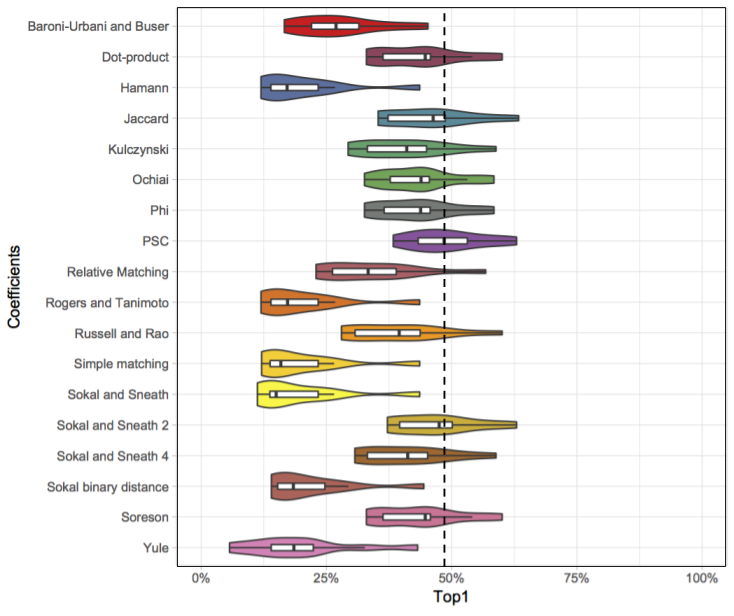
\includegraphics[width=0.7\textwidth]{MCt.png}}	    }
	    \subfigure[Move Method]{\label{fig:plotmmt}%
	    \makebox[\textwidth][c]{
	      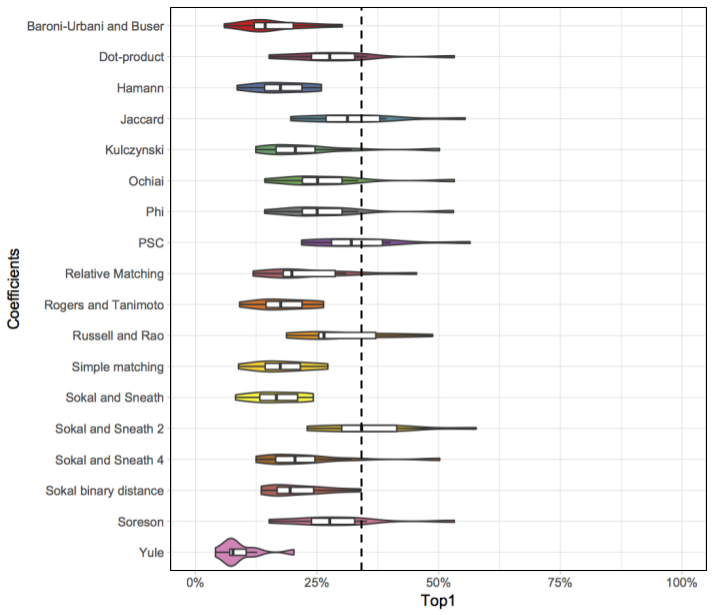
\includegraphics[width=0.7\textwidth]{MMt.png}}
	    }\\
	    \subfigure[Extract Method]{\label{fig:plotemt}%
	    	\makebox[\textwidth][c]{
	      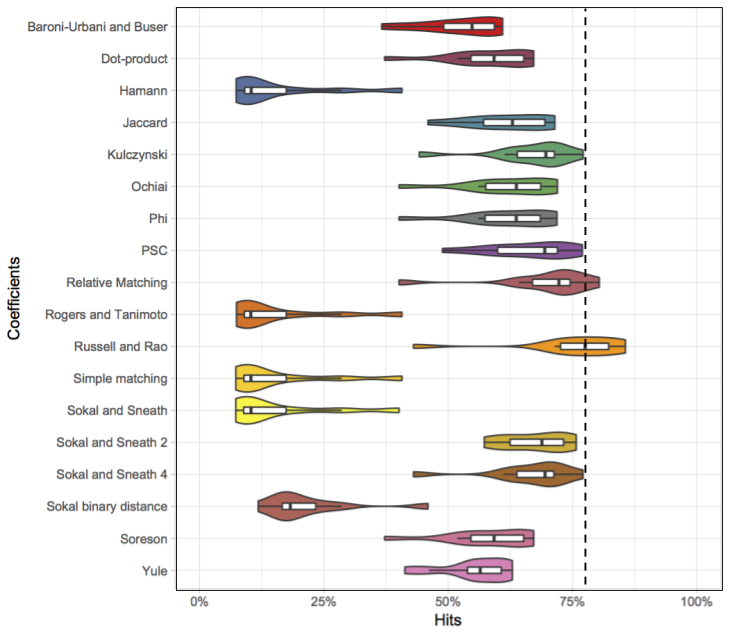
\includegraphics[width=0.7\textwidth]{EMt.png}}
	    }
	  \vspace{-2pt}
	  \caption{Refactorings Plots}
	  \label{fig:violtr}
	  \vspace{-2pt}
\end{figure}

After analyzing and comparing the main existing coefficients, we selected \textit{Simple Matching} to be adapted in order to generate a new coefficient. The \textit{Simple Matching} coefficient has an easy structure to be adapted, defining weights for the variables, thus contributing to obtain good results in the proposal of new coefficients. In contrast, a large part of the analyzed coefficients had already defined weights. Although it was not the best-performing coefficient, the possible weight definition of \textit{Simple Matching} allows simulating coefficients as \textit{Sokal and Sneath 2}, which was the best coefficient in \textit{Move Method} and second best in \textit{Move Class}\footnote{\textit{PSC} was the best coefficient for \textit{Move Class}, however, it was not selected \textcolor{black}{because it englobes elementary arithmetic operations among the variables $a$, $b$, and $c$. Such mathematical relation is out of the scope of this study.}}, as well as \textit{Russell and Rao}, which obtained greater accuracy in \textit{Extract Method}. Additionally, the coefficient considers the universe of dependencies, in contrast to coefficient \textit{PSC}, for instance.


\section{Proposal of New Coefficients}
\label{sec:proposta}

\textcolor{black}{Given the fact that genetic algorithms have nondeterministic execution and results, it becomes a problem to know if their results are satisfactory or even adequate for the expected purpose. In order to address this problem, it was designed an experiment for the proposal of the new coefficients. The experiment consists in a treatment combination with replication, i.e., the repetition of multiple executions in different groups of factor levels. This design is composed by two factors, the initial population size and the number of generations for the genetic algorithm.}

\textcolor{black}{After selecting the \textit{Simple Matching} coefficient to be adapted, several executions of a genetic algorithm is applied to the referred coefficient, having 10 systems of the \textit{Qualitas.class Corpus} as training set.}

\textcolor{black}{The conducted experiment aim to find which candidates resulted in a better value for the objective function. %
%it was defined to maximize the accuracy of the selected algorithm as the optimization objective. 
For this purpose, the genetic algorithm relies on the configuration used in the illustrative example of Section~\ref{sec:exemilus} (see Table~\ref{tab:conf1}). However, in order to find better results and lower the degree of uncertainty, it was defined five configuration groups, with the combination of different factor levels, and replicated five times each, totaling 25 executions. More precisely, each group maintains the original genetic algorithm configuration, changing only the initial population size and the number of generations (the experiment factors), as shown in Table~\ref{tab:conftuk}.} 

\setlength{\tabcolsep}{10pt}
\begin{table}[H]
\vspace{-3pt}
\centering
\caption{Experiment Groups of Factor Level}
\vspace{-8pt}
\label{tab:conftuk}
%\resizebox{\linewidth}{!}{%
%\begin{tabular}{@{}llll@{}}
%\begin{tabular}{p{50.5pt}lp{50.5pt}@{\hspace{6pt}}lll@{}}
\begin{tabular}{lcc}
%\tabucline[1.5pt]{-}
\hline %\hline\noalign{\smallskip}
\rowcolor{gray!50} \textbf{} & \textbf{Population Size} & \textbf{No of Generations} \\ 
\hline %\noalign{\smallskip}\hline %\hline\noalign{\smallskip}
\rowcolor{white}Group 1 & 2000 & 1000  \\ %\hline
\rowcolor{gray!15}Group 2 & 1500 & 1500 \\ %\hline
\rowcolor{white}Group 3 & 500 & 2000 \\ 
\rowcolor{gray!15}Group 4 & 300 & 2500  \\
\rowcolor{white}Group 5 & 100 & 3000 \\ 
\hline %\noalign{\smallskip}\hline
\end{tabular}
%}
\vspace{-6pt}
\end{table}

\textcolor{black}{It is important to clarify that each new proposed coefficient is resulting from a different set of executions of the genetic algorithm (25 executions for each coefficient). Since a single iteration of the genetic algorithm performs thousands of comparisons between code entities to improve results, we argue that this number of executions is satisfactory.}

After generating the set of solutions, in most cases are presented several possibilities that result in the same highest accuracy rate. Therefore, a single solution is selected that shows a greater distance between the mean of similarity indexes that it seeks to maximize with the mean of indexes that it seeks to minimize since a greater distance indicates that the coefficient will tend to maximize and to minimize the similarities correctly in other systems.

Thus, considering the possibility of defining weights to the \textit{Simple Matching} coefficient variables, it was initially simulated as genetic algorithm candidates the weights of \textit{Sokal and Sneath 2} coefficient for \textit{Move Class} and \textit{Move Method} refactorings, as well as \textit{Russell and Rao} weights for \textit{Extract Method} refactorings, which facilitates the selection of new candidates since they were the best results in their respective refactorings. Subsequently, we performed the executions of the genetic algorithm on the 10 systems (training set) in order to obtain more adequate weights for each coefficient variable and to create the new coefficients to be evaluated in the other 101 systems (test set).

\textcolor{black}{Finally, each execution of the experiment was carried out in order to find a higher value for the objective function. Table~\ref{tab:tuktest} shows the values of each execution.}

\begin{table}[tbp]
% \makegapedcells
  \centering
  \caption{Experiment's Objective Function Results}
\vspace{-8pt}
\resizebox*{\linewidth}{!}{%
\footnotesize
    \begin{tabular}{lccccc}
    \hline %\hline\noalign{\smallskip}
    \rowcolor{gray!50}\multicolumn{6}{c}{\textbf{MOVE CLASS}} \\
    \hline %\noalign{\smallskip}\hline %\hline\noalign{\smallskip}
    \rowcolor{gray!25} & Execution~\#1 & Execution~\#2 & Execution~\#3 & Execution~\#4 & Execution~\#5\\
    Group 1 & 3268 & 3176 & 3282 & 3112 & 3198 \\
    \rowcolor{gray!15}Group 2 &  3288 & 3061 & 3241 & 3281 & 3186 \\
    Group 3 &  3273 & 3044 & 3273 & 3171 & 3098 \\
    \rowcolor{gray!15} Group 4 & 3211 & 2989 & 3065 & 3163 & 3177 \\
    Group 5 & 3138 & 3250 & 3151 & \cellcolor{mycolor}\textbf{3382} & 3281 \\
    \hline %\noalign{\smallskip}\hline
     \multicolumn{6}{c}{} \\    

     \hline %\hline\noalign{\smallskip}
    \rowcolor{gray!50}\multicolumn{6}{c}{\textbf{MOVE METHOD}} \\
    \hline %\noalign{\smallskip}\hline %\hline\noalign{\smallskip}
    \rowcolor{gray!25} & Execution~\#1 & Execution~\#2 & Execution~\#3 & Execution~\#4 & Execution~\#5\\
    Group 1 & 9794 & 9736 & 10142 & 9256 & 9915 \\
    \rowcolor{gray!15}Group 2 & 9376 & 10058 & 9794 & 9736 & 10129 \\
    Group 3 & 9060 & 9126 & 9051 & \cellcolor{mycolor}\textbf{10189} & 10075 \\
    \rowcolor{gray!15} Group 4 & 9944 & 9370 & 9995 & 9611 & 9922 \\
    Group 5 & 9890 & 9446 & 9164 & 9892 & 10091 \\
    \hline %\noalign{\smallskip}\hline
     \multicolumn{6}{c}{} \\    
     
    \hline %\hline\noalign{\smallskip}
    \rowcolor{gray!50} \multicolumn{6}{c}{\textbf{EXTRACT METHOD}} \\
    \hline
    \rowcolor{gray!25} & Execution~\#1 & Execution~\#2 & Execution~\#3 & Execution~\#4 & Execution~\#5\\
    Group 1 & 21128 & 21165 & 21217 & 21192 & 21110 \\
    \rowcolor{gray!15}Group 2 & 21173 & 21235 & 21141 & 21229 & 21261 \\
    Group 3 & \cellcolor{mycolor}\textbf{21291} & 21207 & 21135 & 21112 & 21175\\
    \rowcolor{gray!15} Group 4 & 21285 & 21156 & 21262 & 21287 & 21262 \\
    Group 5 & 21145 & 21234 & 21235 & 21290 & 21270 \\
    \hline %\noalign{\smallskip}\hline
    \end{tabular}% 
  }
  \label{tab:tuktest}%
%\vspace{-8pt}  
\end{table}%

In this way, we proposed the following coefficients, where each one corresponds to a type of refactoring code: $PTMC$ for \textit{Move Class} operations, $PTMM$ for \textit{Move Method} operations and $PTEM$ for \textit{Extract Method} operations. The implementation of the genetic algorithm on \textit{Simple Matching} in the defined training set resulted in the first version of the three sought coefficients. The resulting weights $P_{a'}$, $P_{d'}$, $P_{a''}$, $P_b$, $P_c$ and $P_{d''}$, \textcolor{black}{as also the resulting exponents $E_{a'}$, $E_{d'}$, $E_{a''}$, $E_b$, $E_c$ and and $E_{d''}$,} corresponding to the variables $a$ and $d$ of the numerator and $a$, $b$, $c$ and $d$ of the denominator, are reported in Equations~\ref{eq:ptmc},~\ref{eq:ptmm}, and~\ref{eq:ptem}. Thereby, when assigning each weight to the corresponding variable of \textit{Simple Matching}, we have the following proposed coefficients:\\[0.48cm]

\begin{comment}
\begin{table}[ht]
\caption{Proposed coefficients weights}
%\vspace{-8pt}
\centering
\label{tab:pesos}
\resizebox{\linewidth}{!}{%
\scriptsize
\begin{tabular}{lcccccccccccc}
\hline %\hline\noalign{\smallskip}
\rowcolor{gray!50} \textbf{Coefficient} & \textbf{$P_{a'}$ } & \textbf{$E_{a'}$ } & \textbf{$P_{d'}$} & \textbf{$E_{d'}$} & \textbf{$P_{a''}$} & \textbf{$E_{a''}$} & \textbf{$P_b$} & \textbf{$E_b$} & \textbf{$P_c$} & \textbf{$E_c$} & \textbf{$P_{d''}$} & \textbf{$E_{d''}$}\\[0.05cm]
\hline %\noalign{\smallskip}\hline %\hline\noalign{\smallskip}
$PTMC$        & 2.0 & 3.0 & 0.1 & 0.5 & 1.71 & 2.0 & 1.98 & 2.0 & 1.78 & 2.0 & 0.1 & 1.0\\
\rowcolor{gray!15}$PTMM$        & 2.0 & 3.0 & 0.85 & 1.0 & 1.64 & 1.0 & 1.95 & 0.5 & 0.1 & 1.0 & 0.9 & 1.0\\
$PTEM$        & 0.48 & 0.5 & 1.56 & 2.0 & 1.82 & 1.0 & 0.89 & 1.0 & 1.87 & 2.0 & 0.47 & 2.0\\
 \hline %\noalign{\smallskip}\hline
\end{tabular}%
}
%\vspace{0.1cm}
\end{table}
\end{comment}

\begin{equation}
\footnotesize
\textit{$PTMC$}  \texttt{ = }  \frac{2\texttt{a}^{3}  \texttt{ + }  0.1\sqrt{\texttt{d}}}{1.71\texttt{a}^{2}  \texttt{ + }  1.98\texttt{b}^{2}  \texttt{ + }  1.78\texttt{c}^{2}  \texttt{ + }  0.1\texttt{d}}\\
\label{eq:ptmc}
\end{equation}

\begin{equation}
\footnotesize
\textit{$PTMM$} \texttt{ = } \frac{2\texttt{a}^{3} \texttt{ + } 0.85\texttt{d}}{1.64\texttt{a} \texttt{ + } 1.95\sqrt{\texttt{b}} \texttt{ + } 0.1\texttt{c} \texttt{ + } 0.9\texttt{d}}\\
\label{eq:ptmm}
\end{equation}

\begin{equation}
\footnotesize
\textit{$PTEM$} \texttt{ = } \frac{0.48\sqrt{\texttt{a}} \texttt{ + } 1.56\texttt{d}^{2}}{1.82\texttt{a} \texttt{ + } 1.89\texttt{b} \texttt{ + } 1.87\texttt{c}^{2} \texttt{ + } 0.47\texttt{d}^{2}}
\label{eq:ptem}
\end{equation}
\vspace{-0.2cm}

\section{Evaluation of the Proposed Coefficients}
\label{sec:avaliacao}

In order to evaluate the efficiency of the proposed coefficients, we compared the accuracy of the respective coefficients with other 18 coefficients in the literature (Table~\ref{tab:table1}), involving the other 101 systems of the \textit{Qualitas.class Corpus}~(test set). We analyzed and compared each proposed coefficient according to its respective code refactoring, i.e., this section presents a different comparison for  \textit{Move Class}, \textit{Move Method}, and \textit{Extract Method}.\\[-0.2cm]

For the evaluation of the results, we adopted the same analysis approach described in Section~\ref{sec:analise}. Thus, Table~\ref{tab:anal2} reports the results of the accuracy rates of coefficients analyzed for \textit{Move Class} (including $PTMC$), \textit{Move Method} (including $PTMM$), and \textit{Extract Method} (including $PTEM$) refactorings. \textcolor{black}{Again, the analysis considers the median of the sets of means, since some data do not follow a normal distribution}. For space constraints, the detailed table comprehending the results of each of the 101 systems is publicly available at our comparison website\footnote{\url{https://github.com/rterrabh/2018_emse}}.\\[-0.2cm]

%\rowcolors{2}{gray!15}{white}

\begin{table}[tbp]
  \centering
  \caption{Similarity precision of the 19 similarity coefficients (test set)}
 % \resizebox*{\linewidth}{!}{%
  \vspace{-8pt}
  \footnotesize
    \begin{tabular}{lcccccc}
    \hline
    \rowcolor{gray!50}\multicolumn{4}{c}{\textbf{MOVE CLASS}} \\
    \hline
    \rowcolor{gray!25} & \multicolumn{1}{c}{\textbf{Top1}} & \multicolumn{1}{c}{\textbf{Top2}} & \textbf{Top3} \\
    \rowcolor{gray!25} \multirow{-2}[3]{*}[-4.5pt]{\textbf{Coefficient}} & \multicolumn{3}{c}{\textbf{Median}} \\
    Baroni-Urbani and Buser & 36.31\% & 48.65\% & 57.17\% \\[-0.0110cm]
    \rowcolor{gray!15}Dot-product & 49.93\% & 65.22\% & 72.87\% \\[-0.0110cm]
    Hamann & 22.62\% & 32.18\% & 38.77\% \\[-0.0110cm]
    \rowcolor{gray!15}Jaccard & 51.60\% & 67.52\% & 75.48\% \\[-0.0110cm]
    Kulczynski & 46.86\% & 64.15\% & 72.61\% \\[-0.0110cm]
    \rowcolor{gray!15}Ochiai & 49.66\% & 64.94\% & 72.47\% \\[-0.0110cm]
    Phi & 49.39\% & 65.22\% & 72.35\% \\[-0.0110cm]
    \rowcolor{gray!15}PSC & \textit{55.98\%} & \textit{71.26\%} & \textit{77.31\%} \\[-0.0110cm]
    Relative Matching & 36.86\% & 54.35\% & 63.71\% \\[-0.0110cm]
    \rowcolor{gray!15}Rogers and Tanimoto & 22.88\% & 32.18\% & 38.88\% \\[-0.0110cm]
    Russell and Rao & 45.59\% & 61.90\% & 71.31\% \\[-0.0110cm]
    \rowcolor{gray!15}Simple matching & 23.05\% & 33.18\% & 39.23\% \\[-0.0110cm]
    Sokal and Sneath & 22.56\% & 32.25\% & 38.64\% \\[-0.0110cm]
    \rowcolor{gray!15}Sokal and Sneath 2 & 53.35\% & 69.05\% & 76.59\% \\[-0.0110cm]
    Sokal and Sneath 4 & 46.95\% & 63.99\% & 72.54\% \\[-0.0110cm]
    \rowcolor{gray!15}Sokal binary distance & 26.09\% & 35.69\% & 44.36\% \\[-0.0110cm]
    Sorenson & 49.93\% & 65.22\% & 72.87\% \\[-0.0110cm]
    \rowcolor{gray!15}Yule & 26.88\% & 38.64\% & 47.79\% \\[-0.0110cm]
    \rowcolor{mycolor}PTMC & 62.20\% & 71.52\% & 79.45\% \\[-0.0110cm]
    \hline
     \rowcolor{white}\multicolumn{4}{c}{} \\    \hline
    \rowcolor{gray!50}\multicolumn{4}{c}{\textbf{MOVE METHOD}} \\
    \hline
       \rowcolor{gray!25}  & \multicolumn{1}{c}{\textbf{Top1}} & \multicolumn{1}{c}{\textbf{Top2}} & \textbf{Top3} \\
    \rowcolor{gray!25} \multirow{-2}[3]{*}[-4.5pt]{\textbf{Coefficient}} & \multicolumn{3}{c}{\textbf{Median}} \\     
    Baroni-Urbani and Buser & 17.09\% & 25.08\% & 29.97\% \\[-0.0110cm]
    \rowcolor{gray!15}Dot-product & 31.25\% & 41.45\% & 49.23\% \\[-0.0110cm]
    Hamann & 20.21\% & 27.18\% & 31.61\% \\[-0.0110cm]
    \rowcolor{gray!15}Jaccard & 35.43\% & 46.60\% & 53.09\% \\[-0.0110cm]
    Kulczynski & 25.33\% & 36.09\% & 42.79\% \\[-0.0110cm]
    \rowcolor{gray!15}Ochiai & 29.30\% & 41.45\% & 47.49\% \\[-0.0110cm]
    Phi & 29.46\% & 41.29\% & 47.41\% \\[-0.0110cm]
    \rowcolor{gray!15}PSC & 36.71\% & 48.45\% & 55.98\% \\[-0.0110cm]
    Relative Matching & 23.23\% & 34.41\% & 40.39\% \\[-0.0110cm]
    \rowcolor{gray!15}Rogers and Tanimoto & 20.36\% & 27.47\% & 31.81\% \\[-0.0110cm]
    Russell and Rao & 30.70\% & 43.51\% & 49.86\% \\[-0.0110cm]
    \rowcolor{gray!15}Simple matching & 20.25\% & 27.04\% & 31.59\% \\[-0.0110cm]
    Sokal and Sneath & 19.56\% & 26.37\% & 30.46\% \\[-0.0110cm]
    \rowcolor{gray!15}Sokal and Sneath 2 & \textit{38.02\%} & \textit{49.35\%} & \textit{56.04\%} \\[-0.0110cm]
    Sokal and Sneath 4 & 24.35\% & 35.54\% & 42.94\% \\[-0.0110cm]
    \rowcolor{gray!15}Sokal binary distance & 23.75\% & 30.91\% & 35.49\% \\[-0.0110cm]
    Sorenson & 31.25\% & 41.45\% & 49.23\% \\[-0.0110cm]
    \rowcolor{gray!15}Yule & 9.45\% & 17.38\% & 22.25\% \\[-0.0110cm]
    \rowcolor{mycolor}PTMM & 52.89\% & 61.09\% & 64.66\% \\[-0.0110cm]
\hline
    \multicolumn{4}{c}{} \\    \hline
    \rowcolor{gray!50}\multicolumn{4}{c}{\textbf{EXTRACT METHOD}} \\
    \hline
    \rowcolor{gray!25} & \multicolumn{3}{c}{\textbf{Hits}} \\
    \rowcolor{gray!25}\multirow{-2}[3]{*}[-4.5pt]{\textbf{Coefificient}} & \multicolumn{3}{c}{\textbf{Median}} \\
    Baroni-Urbani and Buser & \multicolumn{3}{c}{61.94\%} \\[-0.0110cm]
    \rowcolor{gray!15}Dot-product & \multicolumn{3}{c}{69.62\%} \\[-0.0110cm]
    Hamann & \multicolumn{3}{c}{10.48\%} \\[-0.0110cm]
    \rowcolor{gray!15}Jaccard & \multicolumn{3}{c}{71.73\%} \\[-0.0110cm]
    Kulczynski & \multicolumn{3}{c}{78,36\%} \\[-0.0110cm]
    \rowcolor{gray!15}Ochiai & \multicolumn{3}{c}{72.95\%} \\[-0.0110cm]
    Phi & \multicolumn{3}{c}{72.68\%} \\[-0.0110cm]
    \rowcolor{gray!15}PSC & \multicolumn{3}{c}{76.11\%} \\[-0.0110cm]
    Relative Matching & \multicolumn{3}{c}{82.46\%} \\[-0.0110cm]
    \rowcolor{gray!15}Rogers and Tanimoto & \multicolumn{3}{c}{10.52\%} \\[-0.0110cm]
    Russell and Rao & \multicolumn{3}{c}{\textit{87.93\%}} \\[-0.0110cm]
    \rowcolor{gray!15}Simple matching & \multicolumn{3}{c}{10.48\%} \\[-0.0110cm]
    Sokal and Sneath & \multicolumn{3}{c}{10.32\%} \\[-0.0110cm]
    \rowcolor{gray!15}Sokal and Sneath 2 & \multicolumn{3}{c}{74.67\%} \\[-0.0110cm]
    Sokal and Sneath 4 & \multicolumn{3}{c}{77.27\%} \\[-0.0110cm]
    \rowcolor{gray!15}Sokal binary distance & \multicolumn{3}{c}{16.52\%} \\[-0.0110cm]
    Sorenson & \multicolumn{3}{c}{69.62\%} \\[-0.0110cm]
    \rowcolor{gray!15}Yule & \multicolumn{3}{c}{65.90\%} \\[-0.0110cm]
    \rowcolor{mycolor}PTEM & \multicolumn{3}{c}{88.32\%} \\[-0.0110cm]    \hline
    \end{tabular}%
   % }
    %\vspace{-0.3cm}
  \label{tab:anal2}%
  \vspace*{-8pt}
\end{table}%

\noindent{\bf Move Class}: \textcolor{black}{The proposed coefficient reached higher values compared to the others, having an approximate median of 62.20\%, 71.52\%, and 79.45\% in relation to the similarity rates \textit{Top~\#1},~\textit{\#2}, and~\textit{\#3}. \textit{PSC} presented the second best median among the coefficients analyzed. For \textit{Top~\#1},~\textit{\#2}, and~\textit{\#3}, \textit{PSC} reached, respectively, the accuracy values of 55.98\%, 71.26\% e 77.31\%.} %More importantly, $PTMC$ was 7.88\% higher than \textit{Top~\#1}, 1.62\% than \textit{Top~\#2} and 0.86\% than \textit{Top~\#3} from \textit{PSC}. 

\textcolor{black}{More importantly, when comparing the \textit{Top~\#1} of the coefficients, $PTMC$ presented a statistically significant improvement from 5.23\% to 6.81\%, according to the Wilcoxon Test with a 95\% confidence (\textit{p-value} = ${2.2}^{-16}$)}. %The same happens with \textit{Top~\#2} and \textit{Top~\#3}, with a superiority interval of -0.70\% to  0.89\% and 1.35\% to 3.20\%, respectively (\textit{p-values} = 0.9797 and ${3.539}^{-06}$).} 
%It is also possible to notice an increase of 36.37\%, 34.56\% and 33.52\% in relation to the values of, respectively, \textit{Simple Matching} \textit{Top~\#1}, \textit{Top~\#2} and \textit{Top~\#3}, coefficient of which $PTMC$ was adapted.
\textcolor{black}{Similarly as illustrated in Section~\ref{sec:analise}, Figure~\ref{fig:graph2} presents a violin plot regarding Top~\#1 of each \textit{Move Class} refactoring, in order to provide a complementary analysis between the data.}\\[-0.2cm]

\begin{figure}[ht]
\centering
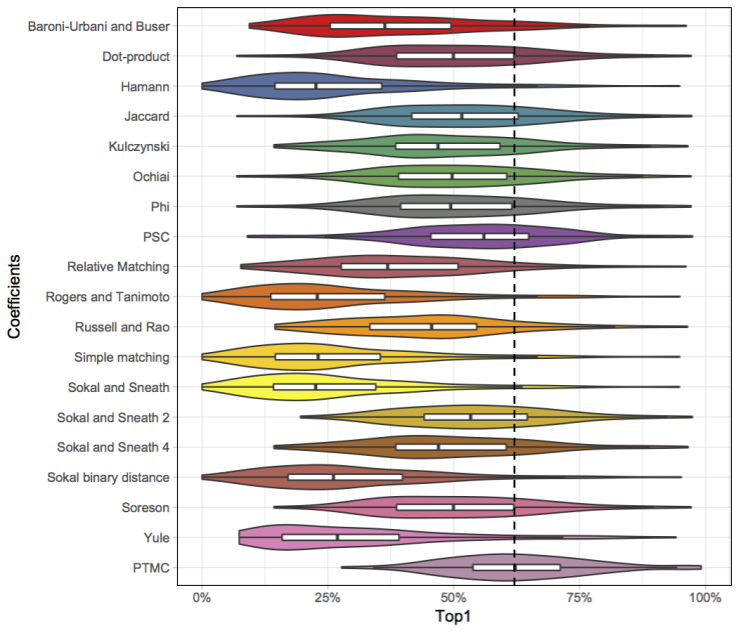
\includegraphics[scale=0.36]{MC.png}
\vspace{-5pt}
\caption{Move Class Plot}
%\vspace{-10pt}
\label{fig:graph2}
\end{figure}

\noindent{\bf Move Method}: \textcolor{black}{$PTMM$ surpassed the other coefficients data in the three cases of similarity rate (\textit{Top~\#1},~\textit{\#2}, and~\textit{\#3}), reaching, respectively, a median of approximately 52.89\%, 61.09\% and 64.66\%. \textit{Sokal and Sneath 2} had the second highest rate where, considering the three cases of similarity rate (\textit{Top~\#1},~\textit{\#2} and~\textit{\#3}), the coefficient reached, respectively, the median values of 38.02\%, 49.35\% and 56.04\%.} %Therefore, it can be concluded that $PTMM$ was 13.39\% better than \textit{Top~\#1} 9.07\% better than \textit{Top~\#2} and 7.83\% better than \textit{Top~\#3} from \textit{Sokal and Sneath 2}. 
\textcolor{black}{Moreover, $PTMM$ presented a statistically significant improvement from 12.33\% to 14.74\%, when comparing \textit{Top~\#1} of the coefficients, according to the Wilcoxon Test with a 95\% confidence (\textit{p-value} = ${2.2}^{-16}$)}. %The same happens with \textit{Top~\#2} and \textit{Top~\#3}, with a superiority interval of 9.67\% to 12.03\% and 7.24\% to 9.48\%, respectively (\textit{p-values} = ${2.2}^{-16}$ and ${2.2}^{-16}$).}
%In addition, once again there was a significant increase in the proposed coefficient in relation to \textit{Simple Matching}, with an increase of 31.26\%, 30.90\% and 32.21\% over the values of \textit{Top~\#1}, \textit{Top~\#2} and \textit{Top~\#3}, respectively.\\[-0.2cm]
\textcolor{black}{Again, Figure~\ref{fig:graph3} presents a violin plot regarding Top~\#1 of each \textit{Move Method} refactoring.}\\[-0.2cm]

\begin{figure}[ht]
\centering
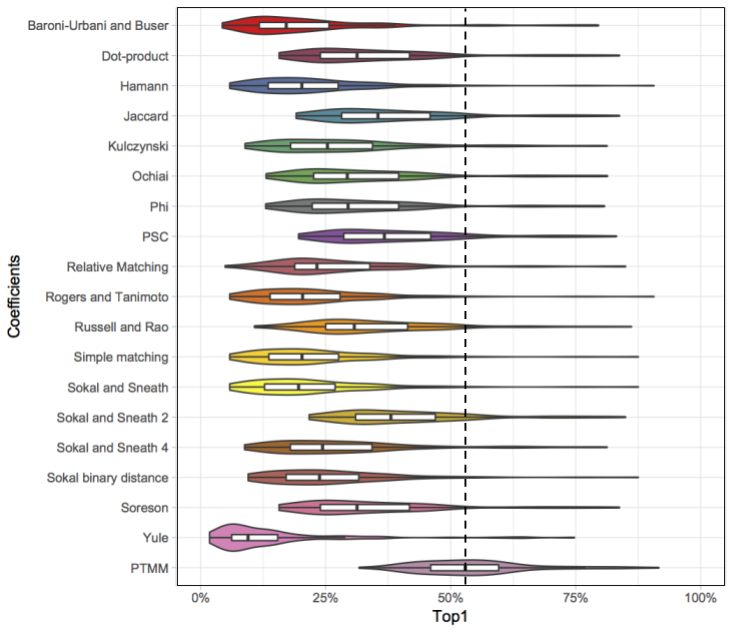
\includegraphics[scale=0.36]{MM.png}
\vspace{-5pt}
\caption{Move Method Plot}
%\vspace{-10pt}
\label{fig:graph3}
\end{figure}

\noindent{\bf Extract Method}: \textcolor{black}{$PTEM$ presented a median of approximately 88.32\%, surpassing the second best coefficient (\textit{Russell and Rao}), which had a median of 87.93\%}. %Thus, $PTEM$ was found to be 0.42\% better in the precision of identification of \textit{Extract Method} refactoring opportunities. And while this difference in the mean is relatively small, $PTEM$ was not the best in only one of the 101 systems analyzed. This small improvement is expected due to the fact that the calculation of blocks and methods similarity consider only the methods of the class itself (as mentioned in Section~\ref{sec: calcsim}), which implies a reduced evaluation spectrum. 
\textcolor{black}{In addition, $PTEM$ presented a statistically significant improvement from 0.24\% to 0.40\% over \textit{Russell and Rao}, according to the Wilcoxon Test with a 95\% confidence (\textit{p-value} = ${2.2}^{-16}$).} 
%It is also relevant to note the increase of 75.17\% in relation to the mean obtained by \textit{Simple Matching}, coefficient of which $PTEM$ was genetically adapted.\\[-0.2cm]
\textcolor{black}{Finally, Figure~\ref{fig:grap4} presents a violin plot regarding each \textit{Extract Method} refactoring.} \\

\begin{figure}[ht]
\centering
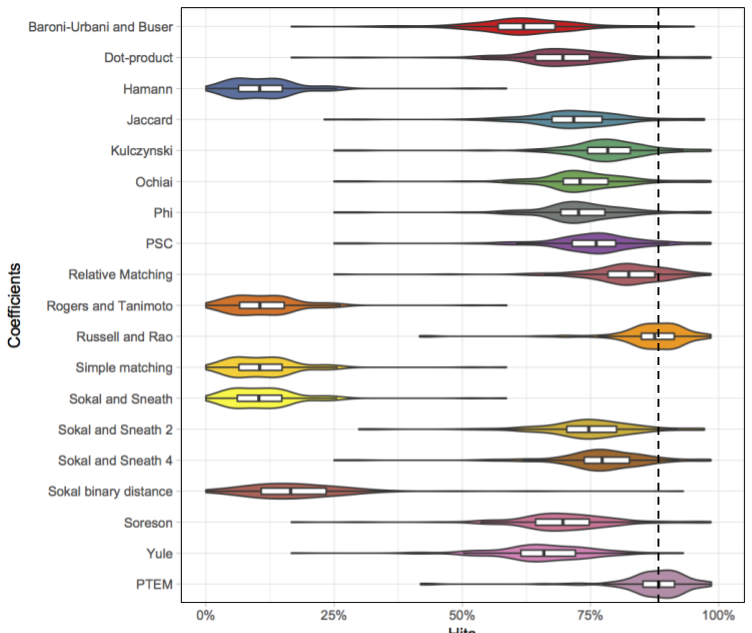
\includegraphics[scale=0.35]{EM.png}
\vspace{-5pt}
\caption{Extract Method Plot}
%\vspace{-10pt}
\label{fig:graph4}
\end{figure}

%\textcolor{black}{Moreover, It is important to mention that, as observed in Table~\ref{tab:anal2}, the proposed coefficients, as well as all the others, presented a normal distribution (p-value \texttt{ > } 0.05) in the 101 systems in a 95\% confidence interval, according to the Wilcoxon~\citep{wilk_shap} and Shapiro~-~Wilk~\citep{wilk_shap} tests.}

\noindent{\bf Threats to validity}: Since the experimental rules play a important role on the results, one could question their underlying design. However, each rule is well well founded and justified at Section~\ref{sec:calcsim}.%Although the execution instructions have been proposed after a series of experimental tests and runs, it cannot be said that the execution instructions described in Section~\ref{sec:calcsim} are complete, since false positives (internal validity) are still possible.

Another important thread is that the experiment described in Section~\ref{sec:proposta} is based in a nondeterministic algorithm and, even considering the replications applied, can lead to a set of different results. Also, changing the factors' values can have different results as well since there are infinite possibilites for them.

Moreover, as it is common in empirical studies in Software Engineering, the results cannot be extrapolated (external validity). Although the test set has a reasonable number of 101 systems, it is important to evaluate the new coefficients in real development scenarios.

\section{Recommendation System}
\label{sec:sistema}

Aiming to apply the new coefficients proposed in this article to identify refactoring opportunities, we developed $AIRP$\footnote{Publicly available from: \url{https://github.com/rterrabh/AIRP}}, a plug-in prototype for IDE Eclipse. %is composed of an architecture based on four main modules::\\[-0.3cm]%A Figura~\ref{fig:diagclasse} ilustra a arquitetura da ferramenta, a qual implementa uma solução baseada em quatro módulos principais:\\[-0.8cm]

For a better understanding of the proposed tool, we executed $AIRP$ in an example involving a modified version (in order to create the refactoring suggestions) of $myAppointments$~\citep{leoterr}, a simple personal information management system with modules $Model$, $View$, $Controller$, and $Util$ (following a MVC architecture).

\textcolor{black}{Figure~\ref{fig:graph} illustrates three examples of suggestions for refactoring identified by $AIRP$. For the modified version of $myAppointments$, class $AngendaDAO$ has a similarity mean value 0.22 higher with the classes of package $myappointments.model.domain$ (\textit{Move Class}), method $loadDriver()$ from class $DB$ has a similarity mean value 0.14 higher with methods from $StringUtils$ (\textit{Move Method}), and finally, method $actionPerformed$ will result in a similarity mean value 0.15 higher with methods from class $AgendaView$ if its second inner block from the second block is extracted to a new method (\textit{Extract Method}).}

\begin{figure}[htbp]
\centering
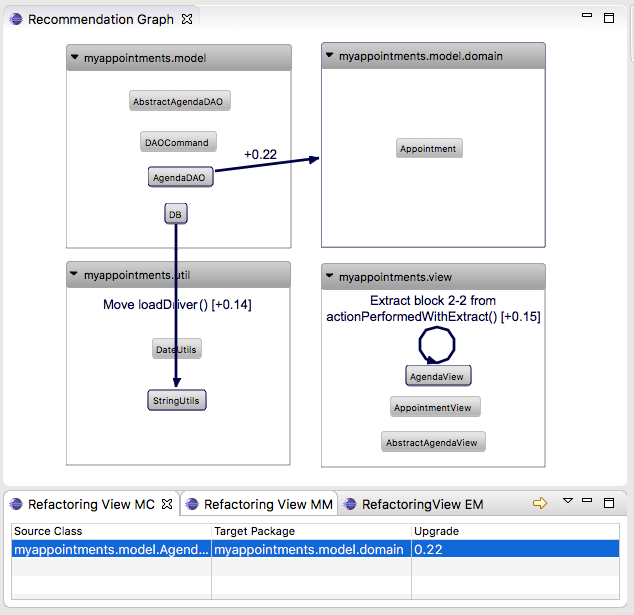
\includegraphics[scale=0.4]{graph.png}
\vspace{-5pt}
\caption{Refactoring opportunity graph}
\vspace{-10pt}
\label{fig:graph}
\end{figure}

%\begin{comment}
%\hspace{0.5cm}
%\begin{figure}[H]
%\centering
%\includegraphics[scale=0.43]{diagclasse.png}
%\vspace{-10pt}
%\caption{Arquitetura do $AIRP$}
%\label{fig:diagclasse}
%\vspace{-15pt}
%\end{figure}
%\hspace{0.5cm}
%\end{comment}

In order to provide the mentioned results, $AIRP$ is composed of an architecture based on four main modules:

\begin{itemize}
\item \noindent{\bf \textit{Dependency Extraction Module}}: Responsible for identifying and storing all dependencies of a class, method, or block. In other words, it identifies the set of types at which a code entity establishes structural dependency. This includes method calling, attribute access, instantiation, variable declaration, annotation, etc. \textcolor{black}{In order to perform such extraction, we used a syntactic analysis through an AST (\textit{Abstract Syntax Tree}) that checks each element in the source code and, if it refers to a dependency to other entities, stores it according to its package, class, method, and/or block.};\\[-0.2cm]

\item \noindent{\bf \textit{Similarity Calculation Module}}: It calculates the structural similarity of a given code entity in the target system. This calculation is performed using the formula of the chosen similarity coefficient, making a comparison between the previously stored dependencies of a given class, method, or block with its respective entity (package, class or, method)\textcolor{black}{, as described in the methodology of this article (See Section~\ref{sec:calcsim}). By default, it uses the $PTMC$, $PTMM$ and $PTEM$ coefficients, although it is possible to select any of the other 18 coefficients presentes in Table~\ref{tab:table1}};\\[-0.2cm]

\item \noindent{\bf \textit{Recommendation Module}}: \textcolor{black}{This module calls the previous one to calculate the resulting similarity of every possible \textit{Move Class}, \textit{Move Method}, and \textit{Extract Method} refactorings in the code.} After calculating similarity, its results are compared with a minimum acceptance index \textcolor{black}{of improvement} specified by the user. If the result is \textcolor{black}{higher} than this user-defined {\em threshold}, a list of suggestions is presented with possible refactoring opportunities. Afterwards, it reports the recommendations for the user analysis, being ordered by their similarity index \textcolor{black}{improvement. If the user does not specify a minimum acceptance index, all refactorings that leads to an improvement are displayed}; and\\[-0.2cm]

%\textcolor{black}{PRINTSCREEN DA LISTA DE SUGESTOES DE REFATORAÇAO}

\item \noindent{\bf \textit{Visualization Module}}: In order to provide more details on the structural organization of the target system, this module generates a refactoring opportunity graph, as illustrated in Figure~\ref{fig:graph}, \textcolor{black}{using the Zest\footnote{\url{https://www.eclipse.org/gef/zest/}} library. This graph contains the implemented architecture and reports all refactorings in the list of suggestions from previous module. The module also highlights the selected refactoring by the user, showing more details about it, and its respective resulting similarity upgrade}. In this way, it makes possible a greater understanding by the user regarding the process performed by the tool, being able to observe the repositioning of involved entities and the architecture resulting from each recommendation.\\[-0.3cm]
\end{itemize}

%Suponha, por exemplo, um sistema com três pacotes $pkg1$, $pkg2$ e $pkg3$ contendo, respectivamente, duas classes $A$ e $B$ com um método cada ($pkg1$~=~\{$A$=\{$m\acute{e}todoA1$\}, $B$=\{$m\acute{e}todoB1$\}\}), uma classe $C$ contendo dois métodos ($pkg2$ = \{$C$=\{$m\acute{e}todoC1$, $m\acute{e}todoC2$\}\}), e uma classe $D$ contendo também dois métodos ($pkg3$ = \{$D$=\{$m\acute{e}todoD1$, $m\acute{e}todoD2$\}\}).

\section{Related Work}
\label{sec:trabrela}

Although it was found only one study regarding the proposal of new similarity coefficients, some studies present methodologies and techniques for the identification of refactoring opportunities, adaptations of existing metrics or empirical studies regarding the concepts discussed in the present article. Considering that the objective of this article is to improve the identification of refactoring opportunities through similarity coefficients, we did not considered studies that do not use such coefficients. The most relevant studies to this article are presented below, according to their categories.\\[-0.2cm]

\noindent{\bf \textit{Proposal of structural similarity coefficients:}} \citet{Naseem2010}~propose a new similarity coefficient aimed at its application in clustering algorithms. In turn, the new proposed coefficient is an adaptation of the \textit{Jaccard} coefficient, called \textit{Jaccard-NM}, whose main difference is the addition of a new variable that considers the universe of analyzed factors, i.e., all the existing factors in the set in which analyzed entities are present. It is important to emphasize that the proposed new similarity coefficient is compared only to the \textit{Jaccard} coefficient, from which it was adapted and in only three systems. On the other hand, this article has an in-depth analysis of the proposed coefficients for a more precise identification in relation to other existing coefficients.\\[-0.2cm]

\noindent{\bf \textit{Empirical studies:}} \citet{2013_seke}~perform a robust evaluation in 111 systems of the base \textit{Qualitas.class Corpus}, involving 18 of the main similarity coefficients. Considering the study purpose, it is fundamental to the accomplishment of this article, considering that the used coefficients and their analyses, besides the approach involving structural dependencies, acted as the main basis for the proposal of new coefficients, as well as their evaluations.

{\citet{szHoke2015automatic}~present a case study where it is discussed whether automatic code refactorings actually improve maintainability of software systems. %Dessa forma, são analisados os impactos de diferentes tipos de refatoração automática em quatro projetos de software em cenários reais de desenvolvimento. São analisadas diversas métricas de qualidade com foco em manutenibilidade, %e.g., LLCOM(\textit{Logical Lines Of Code}), NOA (\textit{Number Of Ancestors}) e CC (\textit{Clone Coverage})
%bem como a aceitação por parte dos desenvolvedores.
Although the study reports that refactorings usually have a positive impact on maintainability, their execution without proper analysis can negatively impact the system. Although it is extremely important to investigate the actual use of automatic refactorings, this article proposes coefficients that identify more precisely refactoring opportunities that may or {\em may not} be amenable to automatic refactoring.}\\[-0.2cm]

\noindent{\bf \textit{Systematic reviews of literature:}} \citet{AlDallal2015231}~presents a systematic review of the literature regarding code refactoring. The study addresses 47 studies on the types of refactoring activities, the different approaches to identify refactoring opportunities, as well as the data sets and the means used to evaluate them. Such review was highly relevant in this article since the performed analyses brought to us the most appropriate approaches to be considered, as well as to better understand the process of identifying code refactoring opportunities, as well as their accomplishment and evaluation.\\[-0.2cm]

\noindent{\bf \textit{Tools for identifying refactoring opportunities:}} \citet{terra2018jmove}~described the proposal of JMove tool, an Eclipse IDE plug-in indicating \textit{Move Method} refactoring opportunities based on the structural similarity coefficient \textit{Sokal and Sneath~2}. The tool, however, involves analysis only of \textit{Move Method}. More importantly, the use of the $PTMM$, coefficient, proposed in this article, could improve accuracy of JMove up to 14.74\%.

\citet{2014_icpc}~proposed JExtract tool, an Eclipse IDE plug-in aimed at identifying \textit{Extract Method} refactoring opportunities based on \textit{Kulczynski} similarity coefficient. JExtract, in turn, focuses only on the \textit{Extract Method} refactoring. Similarly, the use of the $PTEM$ coefficient, proposed in this article, could improve accuracy of JExtract around 9.96\%.

%Ademais, de acordo com a avaliação deste artigo, o uso do coeficiente $PTEM$, proposto neste artigo, poderia melhorar a precisão do JExtract em~9,26\%.

\citet{jdeodoranttse, jdeodoratcsmr}~present the JDeodorant tool, which identifies Code Smells and applies different code refactoring techniques in order to treat them. JDeodorant does not use the similarity comparison between the dependencies of a project. On the other hand, it uses the \textit{Jaccard} coefficient to calculate only the similarity between attributes and methods of the analyzed classes, which can affect its effectiveness since \textit{Jaccard}---although it is one of the most used coefficients in Software Engineering---does not present good accuracy in relation to other existing coefficients.\\[-0.2cm]

Although the analyzed studies show a focus on the identification of code refactoring opportunities or approaches involving structural similarity coefficients, it was not found studies that propose new coefficients aiming at greater accuracy in the identification of such opportunities. Thus, the proposal of new coefficients, based on statistics, robust analyses and comparisons between the main existing similarity coefficients focused on three different types of refactoring, emphasizes the originality of this study.

\section{Conclusion}
\label{sec:conclusao}

Identifying code refactoring opportunities is essential for a developer to maintain a well-defined software architecture, as well as high cohesion and low coupling. Among the existing techniques, several uses the structural similarity calculation. However, the main similarity coefficients proposed in literature are not designed to deal with object-oriented code structures, resulting in low precision and non-realistic rates.

In order to treat this problem, this article presents the proposal of three new structural similarity coefficients in order to provide more precise ways to identification of code refactoring opportunities. For this purpose, we analyzed the main similarity coefficients proposed in literature in a training set of 10 well-designed systems and then, we selected the most adequate coefficient to be adapted and improved. After that, we conducted an experiment with a genetic algorithm and multiple comparisons to propose new coefficients. Finally, we analyzed the proposed coefficients in another 101 well-designed systems. 

This approach resulted in the following similarity coefficients: $PTMC$, for identification of \textit{Move Class} refactoring opportunities; $PTMM$, for \textit{Move Method}; and $PTEM$, for \textit{Extract Method}. The proposed coefficients are more accurate than the hitherto accurate coefficients used to identify refactoring opportunities. In numerical terms, $PTMC$, $PTMM$ and $PTEM$ showed a statistically significant improvement from 5.23\% to 6.81\%, 12.33\% to 14.79\%, and 0.25\% to 0.40\%, respectively, in relation to the second best coefficients. These results can impact in many techniques that uses structural similarity calculation, for example, the precision of the tools JMove and JExtract could be improved up to 14.74\% and 9.96\%, respectively. We also presented $AIRP$, a plug-in for IDE Eclipse to identify refactoring opportunities, that implements the proposed coefficients.

As future studies, it is intended to:
(i)~to use more coefficients in the analysis stage;
(ii)~apply cross-validation techniques; 
(iii)~perform a comparative study among techniques in order to identify refactoring opportunities that use or not similarity coefficients;
{(iv)~propose a single coefficient that meets other types of refactoring;}
and (v)~measure the acceptance degree of new coefficients in real scenarios.

\bibliographystyle{spbasic}
\bibliography{terracopy,refprojeto,refprojeto2}
%\end{spacing}
%\end{document}




% that's all folks
\end{document}